\documentclass[12pt,]{article}
\usepackage[left=1in,top=1in,right=1in,bottom=1in]{geometry}
\newcommand*{\authorfont}{\fontfamily{phv}\selectfont}
\usepackage[]{mathpazo}


  \usepackage[T1]{fontenc}
  \usepackage[utf8]{inputenc}



\usepackage{abstract}
\renewcommand{\abstractname}{}    % clear the title
\renewcommand{\absnamepos}{empty} % originally center

\renewenvironment{abstract}
 {{%
    \setlength{\leftmargin}{0mm}
    \setlength{\rightmargin}{\leftmargin}%
  }%
  \relax}
 {\endlist}

\makeatletter
\def\@maketitle{%
  \newpage
%  \null
%  \vskip 2em%
%  \begin{center}%
  \let \footnote \thanks
    {\fontsize{18}{20}\selectfont\raggedright  \setlength{\parindent}{0pt} \@title \par}%
}
%\fi
\makeatother




\setcounter{secnumdepth}{0}

\usepackage{longtable,booktabs}

\usepackage{graphicx,grffile}
\makeatletter
\def\maxwidth{\ifdim\Gin@nat@width>\linewidth\linewidth\else\Gin@nat@width\fi}
\def\maxheight{\ifdim\Gin@nat@height>\textheight\textheight\else\Gin@nat@height\fi}
\makeatother
% Scale images if necessary, so that they will not overflow the page
% margins by default, and it is still possible to overwrite the defaults
% using explicit options in \includegraphics[width, height, ...]{}
\setkeys{Gin}{width=\maxwidth,height=\maxheight,keepaspectratio}

\title{Nobody expects the Spanish Inquisition: The effect of events on
Australian parliamentary discussion \thanks{Thank you to John Tang, Zach Ward, Tim Hatton, Martine Mariotti, Tianyi
Wang, Matt Jacob, Leslie Root, Jill Sheppard, Matthew Kerby, and Chris
Cochrane for their helpful suggestions. \textbf{Version as of}: 29
September 2018; \textbf{comments welcome}:
\href{mailto:rohan.alexander@anu.edu.au}{\nolinkurl{rohan.alexander@anu.edu.au}}.}  }



\author{\Large Monica Alexander\vspace{0.05in} \newline\normalsize\emph{University of Toronto}   \and \Large Rohan Alexander\vspace{0.05in} \newline\normalsize\emph{Australian National University}  }


\date{}

\usepackage{titlesec}

\titleformat*{\section}{\normalsize\bfseries}
\titleformat*{\subsection}{\normalsize\itshape}
\titleformat*{\subsubsection}{\normalsize\itshape}
\titleformat*{\paragraph}{\normalsize\itshape}
\titleformat*{\subparagraph}{\normalsize\itshape}


\usepackage{natbib}
\bibliographystyle{apsr}
\usepackage[strings]{underscore} % protect underscores in most circumstances



\newtheorem{hypothesis}{Hypothesis}
\usepackage{setspace}

\makeatletter
\@ifpackageloaded{hyperref}{}{%
\ifxetex
  \PassOptionsToPackage{hyphens}{url}\usepackage[setpagesize=false, % page size defined by xetex
              unicode=false, % unicode breaks when used with xetex
              xetex]{hyperref}
\else
  \PassOptionsToPackage{hyphens}{url}\usepackage[unicode=true]{hyperref}
\fi
}

\@ifpackageloaded{color}{
    \PassOptionsToPackage{usenames,dvipsnames}{color}
}{%
    \usepackage[usenames,dvipsnames]{color}
}
\makeatother
\hypersetup{breaklinks=true,
            bookmarks=true,
            pdfauthor={Monica Alexander (University of Toronto) and Rohan Alexander (Australian National University)},
             pdfkeywords = {text analysis, politics, Australia},  
            pdftitle={Nobody expects the Spanish Inquisition: The effect of events on
Australian parliamentary discussion},
            colorlinks=true,
            citecolor=blue,
            urlcolor=blue,
            linkcolor=magenta,
            pdfborder={0 0 0}}
\urlstyle{same}  % don't use monospace font for urls

% set default figure placement to htbp
\makeatletter
\def\fps@figure{htbp}
\makeatother



% add tightlist ----------
\providecommand{\tightlist}{%
\setlength{\itemsep}{0pt}\setlength{\parskip}{0pt}}

\usepackage{amsthm}
\newtheorem{theorem}{Theorem}[section]
\newtheorem{lemma}{Lemma}[section]
\theoremstyle{definition}
\newtheorem{definition}{Definition}[section]
\newtheorem{corollary}{Corollary}[section]
\newtheorem{proposition}{Proposition}[section]
\theoremstyle{definition}
\newtheorem{example}{Example}[section]
\theoremstyle{definition}
\newtheorem{exercise}{Exercise}[section]
\theoremstyle{remark}
\newtheorem*{remark}{Remark}
\newtheorem*{solution}{Solution}
\begin{document}
	
% \pagenumbering{arabic}% resets `page` counter to 1 
%
% \maketitle

{% \usefont{T1}{pnc}{m}{n}
\setlength{\parindent}{0pt}
\thispagestyle{plain}
{\fontsize{18}{20}\selectfont\raggedright 
\maketitle  % title \par  

}

{
   \vskip 13.5pt\relax \normalsize\fontsize{11}{12} 
\textbf{\authorfont Monica Alexander} \hskip 15pt \emph{\small University of Toronto}   \par \textbf{\authorfont Rohan Alexander} \hskip 15pt \emph{\small Australian National University}   

}

}








\begin{abstract}

    \hbox{\vrule height .2pt width 39.14pc}

    \vskip 8.5pt % \small 

\noindent Government policy is partly driven by parliamentary discussion.
Conversely, that same discussion can indicate a government's priorities.
But major events--both expected, such as an election, and unexpected,
such as a recession or terrorist attack--can affect the course of
parliamentary discussion. In this paper, we systematically analyse how
parliamentary discussion changes in response to different types of
events in Australian history. We compile a dataset of what was said in
Australian state and federal parliaments from the mid-1800s through to
2017 based on available public records. We use a structural text model
to reduce the dimensionality of the text and to impose prior knowledge
such as correlation between days and changes over time. We then examine
the effect of various events. We find that: 1) changes of government are
associated with topic changes only when there is also a change of the
party in power; and 2) economic events, such as financial crises, have
significant and persistent effects. Our findings have implications for
how we think about the longer-term trajectory of government policy as
the media cycle becomes increasingly focused on short-term events.


\vskip 8.5pt \noindent \emph{Keywords}: text analysis, politics, Australia \par

    \hbox{\vrule height .2pt width 39.14pc}



\end{abstract}


\vskip 6.5pt


\noindent  \section{Introduction}\label{introduction}

New governments often go to some trouble to be different to the
governments they replace. For instance, Kevin Rudd's apology to
Indigenous Australians was not supported by his predecessor John Howard,
and then one of Tony Abbott's first acts was to repeal his predecessor
Kevin Rudd's carbon tax. Similarly, significant events such as the 9/11
attacks or the Great Recession have often altered the course of a
government. However it is not so clear which events drive changes, for
how long these changes persist, and what was given up due to the change.

In this paper we examine text records of what was said in Australian
state and federal parliaments from the mid-1800s through to 2017. We use
the Structural Topic Model (STM) of \citet{RobertsStewartAiroldi2016}
for dimensionality reduction and to impose structure such as correlation
between days and changes over time. We then examine changes at various
types of events, including: changes in government; changes in the
political environment (as defined by polling or other results); changes
in economic conditions; and other significant events (such as the 9/11
attacks or the Bali bombings).

We find \textbf{{[}INSERT RESULTS{]}}.

Our paper applies a topic model to a dataset of larger-scale
parliamentary text records from multiple Australian parliaments. Our
work fits into a growing literature that considers text as an input to
more usual quantitative techniques, rather than requiring separate
analysis. While using text as data has well-known shortcomings, it
allows larger-scale analysis that would not be viable using
less-automated approaches and so it can identify patterns that may
otherwise be overlooked.

\section{Data}\label{data}

\subsection{Parliamentary text data}\label{parliamentary-text-data}

Following the example of the UK a daily text record called Hansard of
what was said in Australian parliaments has been made available since
their establishment.\footnote{While Hansard is not necessarily verbatim,
  it is considered close enough for text-as-data purposes. For instance,
  \citet{Mollin2008} found that in the case of the UK Hansard the
  differences would only affect specialised linguistic analysis.
  \citet{Edwards2016} examined Australia, New Zealand and the UK, and
  found that changes were usually made by those responsible for creating
  the Hansard record, instead of the parliamentarians.} Earlier work on
the influence of parliaments, such as \citet{ZandenBuringhBosker2012} or
\textbf{{[}ANOTHER REFERENCE - Maybe Frank Fisher `Reframing Public
Policy'?{]}}, often examined broader activity measures such as counts of
sitting days. This allowed for long time frames and wide comparisons.
But analysing Hansard records and their equivalents directly are an
increasingly viable and popular source of data as new methods and
reduced computational costs make larger-scale analysis easier,
complementing other measures.

The digitisation of the Canadian Hansard, \citet{BeelenEtc2017}, allowed
\citet{RheaultCochran2018} to examine ideology and party polarisation in
Britain and Canada. In the UK, \citet{Duthie2016} analysed Hansard
records to examine which politicians made supportive or aggressive
statements toward other politicians between 1979 and 1990 and
\citet{PetersonSpirling2018} examined polarisation. And as digitisation
methods improve older UK records can be analysed, for instance
\citet{Dimitruk2018} considers the effect of estate bills on
prorogations in seventeenth century England. In New Zealand,
\citet{Curran2017} modelled the topics discussed between 2003 and 2016,
and \citet{Graham2016} examined unparliamentary language between 1890
and 1950. And in the US \citet{GentzkowShapiroTaddy2018} examine
congressional speech records from 1873 to 2016 to find that partisanship
has risen in the past few decades.

Australian Hansard records have been analysed for various purposes. For
instance, \citet{Rasiah2010} examined Hansard records for the Australian
House of Representatives to examine whether politicians attempted to
evade questions about Iraq during February and March 2003. And
\citet{GansLeigh2012} examined Australian Hansard records to associate
mentions by politicians of certain public intellectuals with neutral or
positive sentiment.

Australian parliaments generally make their daily Hansard records
available online as PDFs and these are considered the official release.
An example of what a page of Hansard looks like is included in Appendix
\textbf{{[}ADD NUMBERING{]}}. There is a more limited set of XML records
available in some cases.\footnote{Tim Sherratt makes these XML records
  available as a single download and also presents them in a website
  (\url{http://historichansard.net/}) that can be used to explore
  Commonwealth Hansard records from 1901 to 1980. Commonwealth XML
  records from 1998 to 2014 are available from Andrew Turpin's website,
  and from 2006 through to today from Open Australia's website. The
  records can also be downloaded from the Australian Hansard website.}
There are 65,000 \textbf{{[}UPDATE{]}} Hansard records publicly
available across the state and federal parliaments (Table
\ref{tab:yearsusedtable}) \textbf{{[}UPDATE NUMBERING{]}}. As with any
larger-scale data process, there are various issues with some of the
PDFs and the known ones are detailed in Appendix \textbf{{[}ADD
NUMBERING{]}}.\footnote{The NSW Legislative Council was established
  earlier than 1856, however the earlier Hansard records have not been
  through an independent OCR process and were not used in this paper.
  However, the Google Tesseract OCR engine as implemented by
  \citet{Ooms2018tesseract} provided useful data and these could be used
  in the future.}

\begin{table}

\caption{\label{tab:yearsusedtable}Hansard records used}
\centering
\fontsize{12}{14}\selectfont
\begin{tabular}[t]{lrrr}
\toprule
Parliament & House & Years used & Number of records\\
\midrule
Commonwealth & House of Representatives & 1901 - 2017 & 7873\\
 & Senate & 1901 - 2017 & TBD\\
Queensland & Legislative Assembly & 1860 - 2017 & 9699\\
 & Legislative Council & 1860 - 1922 & 4156\\
New South Wales & Legislative Assembly & 1856 - 2017 & TBD\\
\addlinespace
 & Legislative Council & 1856 - 2017 & TBD\\
Victoria & Legislative Assembly & 1856 - 2017 & TBD\\
 & Legislative Council & 1851 - 2017 & TBD\\
Tasmania & House of Assembly & 1856 - 2017 & TBD\\
 & Legislative Council & 1856 - 2017 & TBD\\
\addlinespace
South Australia & House of Assembly & 1857 - 2017 & TBD\\
 & Legislative Council & 1840 - 2017 & TBD\\
Western Australia & Legislative Assembly & 1890 - 2017 & TBD\\
 & Legislative Council & 1832 - 2017 & TBD\\
\bottomrule
\end{tabular}
\end{table}

The formatting of the Hansard records changes between the different
parliaments and over time. We use R scripts to convert the PDFs into
daily text records.\footnote{An example of the workflow and some
  reduced-detail scripts are provided in Appendix \textbf{{[}ADD
  NUMBERING{]}}.} These scripts are primarily based on: the
\texttt{PDFtools} package of \citet{Ooms2018pdftools}; the
\texttt{tidyverse} package of \citet{Wickham2017}; the \texttt{tm}
package of \citet{FeinererHornik2018}; the \texttt{lubridate} package of
\citet{GrolemundWickham2011}; and the \texttt{stringi} package of
\citet{Gagolewski2018}. The functions of those packages are supported
by: the \texttt{furrr} package of \citet{VaughanDancho2018}; and the
\texttt{tictoc} package of \citet{Izrailev2014}. Some error is
introduced at this stage because many of the records are in a two-column
format that need to be separated, and the PDF parsing is not always
accurate especially for older records. An example of the latter issue is
that `the' is often parsed as `thc'. These errors are fixed when they
occur at scale and can be identified. One way to provide assurance that
mistakes in older records are not driving the results is to analyse the
percentage of stop-words in each record over time. This details of this
are provided in Appendix \textbf{{[}ADD NUMBERING{]}} and suggest that
there is no significant difference in the quality of the parsing over
time. The \texttt{hunspell} package of \citet{Ooms2017} is also used to
help find spelling issues.

These daily records are the main level at which we consider the data in
this paper, but the daily records are also further divided into
individual-level records. Sometimes these are just short interjections
or notes that are not specific to any particular politician, such as
`Honourable members interjecting'. The high dimensional nature of text
data means that the appropriate analysis data are research-question
specific and datasets need to be tidied toward that. For instance, in
our paper interjections are not important because they do not usually
contribute much to defining the topics being discussed. But they are
interesting in their own right and \citet{Whyte2017} analysed them in a
Canadian context for the period 1926 to 2015 to find that female MPs
were more likely to be interrupted than male MPs.

Usually the disaggregation into individual-level records is done by
identifying politicians' names in particular patterns. For instance,
when Hansard is indicating that a particular person is speaking, as
opposed to being mentioned (for more on the political effect of being
mentioned see \citet{Alexander2018}), often the name is in upper case,
for instance `Mr WHITLAM' or `Mr MENZIES'; followed by a dash or colon;
or are next to some title within brackets. There is substantial
variation in how the person making a statement is identified. Again some
error is introduced at this stage because of inconsistencies over time
and between the parliaments. There is considerable variance but on
average each daily record had 250 \textbf{{[}UPDATE{]}} individual-level
records, resulting in roughly 15 million rows \textbf{{[}UPDATE{]}}
across the state and federal parliaments.

Text usually needs to be pre-processed before topic models can be used.
The specific steps that we take are to remove numbers and punctuation
and to change all the words to lower case. Then the sentences are
deconstructed and each word considered individually. In addition to the
packages already mentioned, in this step the R scripts to do this use
the \texttt{tidytext} R package of \citet{SilgeRobinson2016}.
\textbf{{[}Need to bundle\_ngrams i.e.~New Zealand is new\_zealand.{]}}

\subsection{Additional information}\label{additional-information}

Data from other sources are useful to complement the parliamentary text
data. For instance, although the name, party, and division represented
are contained in Hansard records they are inconsistent. Also non-Hansard
information about the politicians informs our analysis. This includes:
date of birth and date of death; sex; date of entry to parliament and
exit from parliament; some aspects of their pre- and post-parliamentary
career; some aspects of their parliamentary career, such as ministry
appointments; and electoral information such as primary and
two-party-preferred results.

The main sources for this additional supplementary information are the
handbooks supplied by the various parliaments. However these had many
errors and were supplemented by data from the Australian Dictionary of
Biography and Wikipedia.\footnote{An example of the additional
  information is provided in Appendix \textbf{{[}ADD NUMBERING{]}}.} The
source for the electoral results is the Australian Electoral Commission
and Adam Carr's Australian Election Archive.

\section{Model}\label{model}

The main model that we use in this paper is the Structural Topic Model
(STM) as implemented by the \texttt{stm} R package of
\citet{RobertsStewartAiroldiRPackage}. In a similar way to
\citet{MuellerRauh2018}, we use these topics to analyse the effect of
various events. In Appendix \textbf{{[}ADD NUMBERING{]}}, we include an
alternative approach that follows \citet{Taddy2015} by using word2vec,
which more closely uses words, rather than topics, as an input.

The basis of the STM is the Latent Dirichlet Allocation (LDA) model of
\citet{Blei2003latent}. In this section we provide a brief overview of
both the LDA model and the STM. We consider the outputs of the topic
model as reduced dimension inputs that can be analysed.

\subsection{Latent Dirichlet
Allocation}\label{latent-dirichlet-allocation}

Although more- or less-fine levels of analysis are possible, but here we
are primarily interested in considering a day's topics. This means that
each day's Hansard record needs to be classified by its topics.
Sometimes Hansard records includes titles that make the topic clear. But
not every statement has a title and the titles do not always define
topics in a well-defined and consistent way, especially over longer time
periods. One way to get consistent estimates of the topics discussed in
Hansard is to use the LDA method of \citet{Blei2003latent}, for instance
as implemented by the R \texttt{topicmodels} package of
\citet{Grun2011}.

The key assumption behind the LDA method is that each day's text, `a
document', in Hansard is made by speakers who decide the topics they
would like to talk about in that document, and then choose words,
`terms', that are appropriate to those topics. A topic could be thought
of as a collection of terms, and a document as a collection of topics,
where these collections are defined by probability distributions. The
topics are not specified \emph{ex ante}; they are an outcome of the
method. In this sense, this approach can be considered unsupervised
machine learning. Terms are not necessarily unique to a particular
topic, and a document could be about more than one topic. This provides
more flexibility than other approaches such as a strict word count
method. The goal is to have the words found in each day's Hansard group
themselves to define topics.

As applied to Hansard, the LDA method considers each statement to be a
result of a process where a politician first chooses the topics they
want to speak about. After choosing the topics, the speaker then chooses
appropriate words to use for each of those topics. More generally, the
LDA topic model works by considering each document as having been
generated by some probability distribution over topics. Similarly, each
topic could be considered a probability distribution over terms. To
choose the terms used in each document the speaker picks terms from each
topic in the appropriate proportion. Figures
\ref{fig:topicsoverdocuments} and \ref{fig:topicsoverterms} in Appendix
\textbf{{[}ADD NUMBERING{]}} illustrates an example with five topics,
two documents, and ten terms.

Following \citet{BleiLafferty2009}, \citet{blei2012} and
\citet{GriffithsSteyvers2004}, the process by which a document is
generated is more formally considered to be:

\begin{enumerate}
\def\labelenumi{\arabic{enumi}.}
\tightlist
\item
  There are \(1, 2, \dots, k, \dots, K\) topics and the vocabulary
  consists of \(1, 2, \dots, V\) terms. For each topic, decide the terms
  that the topic uses by randomly drawing distributions over the terms.
  The distribution over the terms for the \(k\)th topic is \(\beta_k\).
  Typically a topic would be a small number of terms and so the
  Dirichlet distribution with hyperparameter \(0<\eta<1\) is used:
  \(\beta_k \sim \mbox{Dirichlet}(\eta)\).\footnote{The Dirichlet
    distribution is a variation of the beta distribution that is
    commonly used as a prior for categorical and multinomial variables.
    If there are just two categories, then the Dirichlet and the beta
    distributions are the same. In the special case of a symmetric
    Dirichlet distribution, \(\eta=1\), it is equivalent to a uniform
    distribution. If \(\eta<1\), then the distribution is sparse and
    concentrated on a smaller number of the values, and this number
    decreases as \(\eta\) decreases. A hyperparameter is a parameter of
    a prior distribution.} Strictly, \(\eta\) is actually a vector of
  hyperparameters, one for each \(K\), but in practice they all tend to
  be the same value.
\item
  Decide the topics that each document will cover by randomly drawing
  distributions over the \(K\) topics for each of the
  \(1, 2, \dots, d, \dots, D\) documents. The topic distributions for
  the \(d\)th document are \(\theta_d\), and \(\theta_{d,k}\) is the
  topic distribution for topic \(k\) in document \(d\). Again, the
  Dirichlet distribution with the hyperparameter \(0<\alpha<1\) is used
  here because usually a document would only cover a handful of topics:
  \(\theta_d \sim \mbox{Dirichlet}(\alpha)\). Again, strictly \(\alpha\)
  is vector of length \(K\) of hyperparameters, but in practice each is
  usually the same value.
\item
  If there are \(1, 2, \dots, n, \dots, N\) terms in the \(d\)th
  document, then to choose the \(n\)th term, \(w_{d, n}\):

  \begin{enumerate}
  \def\labelenumii{\alph{enumii}.}
  \tightlist
  \item
    Randomly choose a topic for that term \(n\), in that document \(d\),
    \(z_{d,n}\), from the multinomial distribution over topics in that
    document, \(z_{d,n} \sim \mbox{Multinomial}(\theta_d)\).
  \item
    Randomly choose a term from the relevant multinomial distribution
    over the terms for that topic,
    \(w_{d,n} \sim \mbox{Multinomial}(\beta_{z_{d,n}})\).
  \end{enumerate}
\end{enumerate}

Given this set-up, the joint distribution for the variables is
(\citet{blei2012}, p.6):
\[p(\beta_{1:K}, \theta_{1:D}, z_{1:D, 1:N}, w_{1:D, 1:N}) = \prod^{K}_{i=1}p(\beta_i) \prod^{D}_{d=1}p(\theta_d) \left(\prod^N_{n=1}p(z_{d,n}|\theta_d)p\left(w_{d,n}|\beta_{1:K},z_{d,n}\right) \right).\]

Based on this document generation process the analysis problem,
discussed next, is to compute a posterior over \(\beta_{1:K}\) and
\(\theta_{1:D}\), given \(w_{1:D, 1:N}\). This is intractable directly,
but can be approximated (\citet{GriffithsSteyvers2004} and
\citet{blei2012}).

After the documents are created, they are all that we have to analyse.
The term usage in each document, \(w_{1:D, 1:N}\), is observed, but the
topics are hidden, or `latent'. We do not know the topics of each
document, nor how terms defined the topics. That is, we do not know the
probability distributions of Figures \ref{fig:topicsoverdocuments} or
\ref{fig:topicsoverterms}. In a sense we are trying to reverse the
document generation process -- we have the terms and we would like to
discover the topics.

If the earlier process around how the documents were generated is
assumed and we observe the terms in each document, then we can obtain
estimates of the topics (\citet{SteyversGriffiths2006}). The outcomes of
the LDA process are probability distributions and these define the
topics. Each term will be given a probability of being a member of a
particular topic, and each document will be given a probability of being
about a particular topic. That is, we are trying to calculate the
posterior distribution of the topics given the terms observed in each
document (\citet{blei2012}, p.~7):
\[p(\beta_{1:K}, \theta_{1:D}, z_{1:D, 1:N} | w_{1:D, 1:N}) = \frac{p\left(\beta_{1:K}, \theta_{1:D}, z_{1:D, 1:N}, w_{1:D, 1:N}\right)}{p(w_{1:D, 1:N})}.\]

Gibbs sampling or the variational expectation-maximization algorithm can
be used to approximate the posterior. A summary of these approaches is
provided in Appendix \textbf{{[}ADD NUMBERING{]}}. The choice of the
number of topics, \emph{k}, drives the results and must be specified
\emph{a priori}. If there is a strong reason for a particular number,
then this can be used. Otherwise, one way to choose an appropriate
number is to use cross validation.

One weakness of the LDA method is that it considers a `bag of words'
where the order of those words does not matter (\citet{blei2012}). It is
possible to extend the model to reduce the impact of the bag-of-words
assumption and add conditionality to word order. Additionally,
alternatives to the Dirichlet distribution can be used to extend the
model to allow for correlation. For instance, in Hansard topics related
the army may be expected to be more commonly found with topics related
to the navy, but less commonly with topics related to banking. This
motivates the use of the Structural Topic Model, described in the next
section.

\subsection{Structural Topic Model}\label{structural-topic-model}

The distinguishing aspect of the Structural Topic Model (STM) of
\citet{RobertsStewartAiroldi2016} is that it considers more than just a
document's content when constructing topics. For instance, we generally
have some information about the author and the date that a document was
created. In the case of Hansard, we know who was speaking and the date
they spoke. The STM allows this additional information to affect the
construction of topics, though influencing either topical prevalence or
topical content. That said, the assumption that there is some document
generation process is the same as the LDA method, it is just that this
process now includes metadata.

The STM is set-up to most easily include metadata to do with prevalence
and content. Prevalence relates to the topic proportions in each
document. For instance, we expect that topics related to the reasons for
Federation, such as tariffs and trade, should be more prevalent in those
earlier years than later. Similarly, we may expect topics to do with
terrorism to be more prevalent in recent years. Content relates to the
words that make up each topic. For instance, there are changes in the
use of language over the period for which we have data, and it would be
better for these to not be responsible for defining different topics
rather than being part of the same topic. The prevalence meta-data for
the \(d\)th document are in \(X_d\), which has one column for each
aspect. For instance, if there were 10 documents and each had a date and
an author, then \(X\) would be \(10\times 2\). Similarly, the content
meta-data are

As with LDA, the process assumed to generate the documents is the key
aspect as this will be reversed to estimate the topics. The document
generation process of \citet{Blei2003latent} discussed earlier, is
slightly modified by \citet{RobertsStewartAiroldi2016} for the STM:

\begin{enumerate}
\def\labelenumi{\arabic{enumi}.}
\item
  As with LDA, the topic distributions, that is, the proportion of a
  document dedicated to a topic, for the \(d\)th document are
  \(\theta_d\), and \(\theta\) is a vector with length \(D\). In
  contrast to LDA, this is a drawn from a logistic-normal distribution,
  parameterised such that the mean of that distribution, \(\mu\), is
  affected by a vector of document covariates, \(X_d\) (following
  \citet{RobertsStewartTingley2018}, p.3):
  \[\theta_d|X_d\gamma\Sigma \sim \mbox{Logistic Normal}(\mu = X_d\gamma, \Sigma)\]
\item
  To decide the distribution over terms for each topic, \(\beta_{d,k}\),
  start with some baseline distribution over the terms, \(m\).
  Topic-\(k\)-specific deviations from this are controlled by
  \(\kappa_k^{(t)}\), deviations due to the document meta-data are
  controlled by \(\kappa_{y_d}^{(c)}\), and the interaction between
  these two deviations is controlled by \(\kappa_{y_d,k}^{(i)}\):
  \[\beta_{d,k}\propto \mbox{exp}\left(m+\kappa^{(t)}_{k} + \kappa_{y_d}^{(c)} + \kappa_{y_{d}k}^{(i)}\right) \]
\item
  Then if there are \(n\) terms in the \(d\)th document, then to choose
  the \(n\)th term, \(w_{d,n}\):

  \begin{enumerate}
  \def\labelenumii{\alph{enumii}.}
  \tightlist
  \item
    Randomly choose a topic for that term from the document-specific
    multinomial distribution over topics.
  \item
    Randomly choose a term from the topic-specific multinomial
    distribution over terms.
  \end{enumerate}
\end{enumerate}

We primarily implement the STM on the daily-level parliamentary text
data described earlier using the \texttt{stm} R package of
\citet{RobertsStewartAiroldiRPackage}. We consider both topic prevalence
and content to be functions of time. The choice of the number of topics
to use in the model is a situation-specific compromise. We use standard
diagnostic techniques with cross validation to decide on 80
\textbf{{[}UPDATE AS APPROPRIATE{]}} topics. More detail on this
selection process is available in Appendix \textbf{{[}ADD NUMBERING{]}}.

Figure \ref{fig:exampletopics} illustrates an output of the STM. This
illustrative model only considers data from the House of Representatives
between 1901 and 2017. It shows how each day's parliamentary discussion
can be allocated to one of ten topics and highlights how the prominence
of these topics changes over time. \textbf{{[}RUN AND GRAPH AN ACTUAL
10-TOPIC MODEL - THESE DATA ARE JUST SUMMED FROM THE GENERAL ONE!.{]}}

\begin{figure}
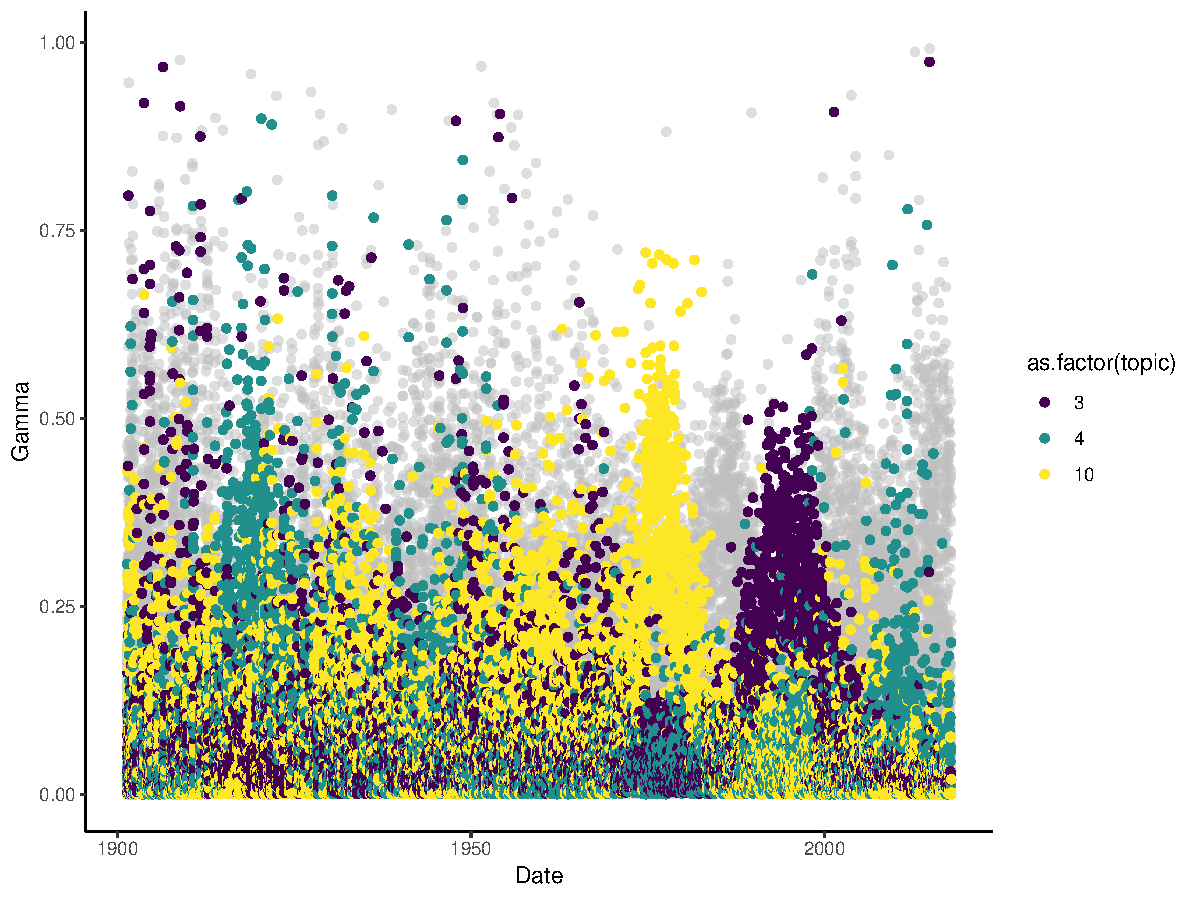
\includegraphics[width=1\linewidth]{/Users/rohanalexander/Documents/phd/hansard/outputs/figures/topics_example} \caption{Estimated 10-topic-proportion}\label{fig:exampletopics}
\end{figure}

\subsubsection{Considering events}\label{considering-events}

We are interested in the effect of political, economic, and other events
on Australian parliamentary discussion. Political events are those
related to a change of government or an election. Economic events are
defined by substantial changes in various economic measures, such as the
onset of the Great Depression or the Great Recession. Other events are
those such as the 9/11 attacks, or the Bali Bombing. The full list of
events that we consider is detailed in Appendix \textbf{{[}ADD
NUMBERING{]}}.

There are many ways to statistically consider the effect of events. One
way would be to ignore the time series aspect and just group the topic
proportions by each event and then run multinomial tests for whether the
groups are different. Another would be to consider some type of
multinomial logistic regression. Options that would take advantage of
the time series nature of our data include: autoregressive moving
average (ARMA) models which can be used to test for structural breaks
\textbf{{[}REFERENCE?{]}}; or splines could be fit with specific knot
placements and then cross validation used to compare the RSS with a more
general splines model.

\textbf{{[}MONICA - LOOK AT THESE OR OTHER OPTIONS AND DECIDE ON A WAY.
NEEDS TO ALLOW FOR SHORT AND LONG RUN AND ALSO ALLOW COINCIDENCE OF
EVENTS. WE ONLY CONSIDER 20 TOPICS BELOW, BUT THAT'S UNDERDONE AND THE
METHODS NEED TO ALLOW FOR MORE.{]}}

We currently consider events in two ways. The first is graphically,
grouping each of the daily topic proportions by the events and isolating
the topics. This illustrates the differences between the topics. The
second is by including incrementing variables in the prevalence metdata.
This groups each day by events and we can then conduct significance
tests. Unfortunately both of these do not consider short-term effects.

\textbf{{[}Use tf-idf between them as illustrative instead? Use that
other measure of difference?{]}}

\section{Results}\label{results}

We are interested in considering the effect of various events on what is
talked about in Australia's parliaments. Each of those parliaments are
treated independently here. Future work could expand the model to better
understand, and allow, for correlation between them.

We consider four types of events and group the day's topic proportions
by these events. One unfortunate effect of this is that we only allow an
event to have a long-run effect and ignore short-run effects. Another is
that we ignore coincidence of events.

Figure \ref{fig:electionsevents} shows the grouping by election. If
elections had significant effects on the discussion in parliament then
there would be considerable change between groups. However changes
generally appear to be longer-term rather than election to election.

\begin{figure}
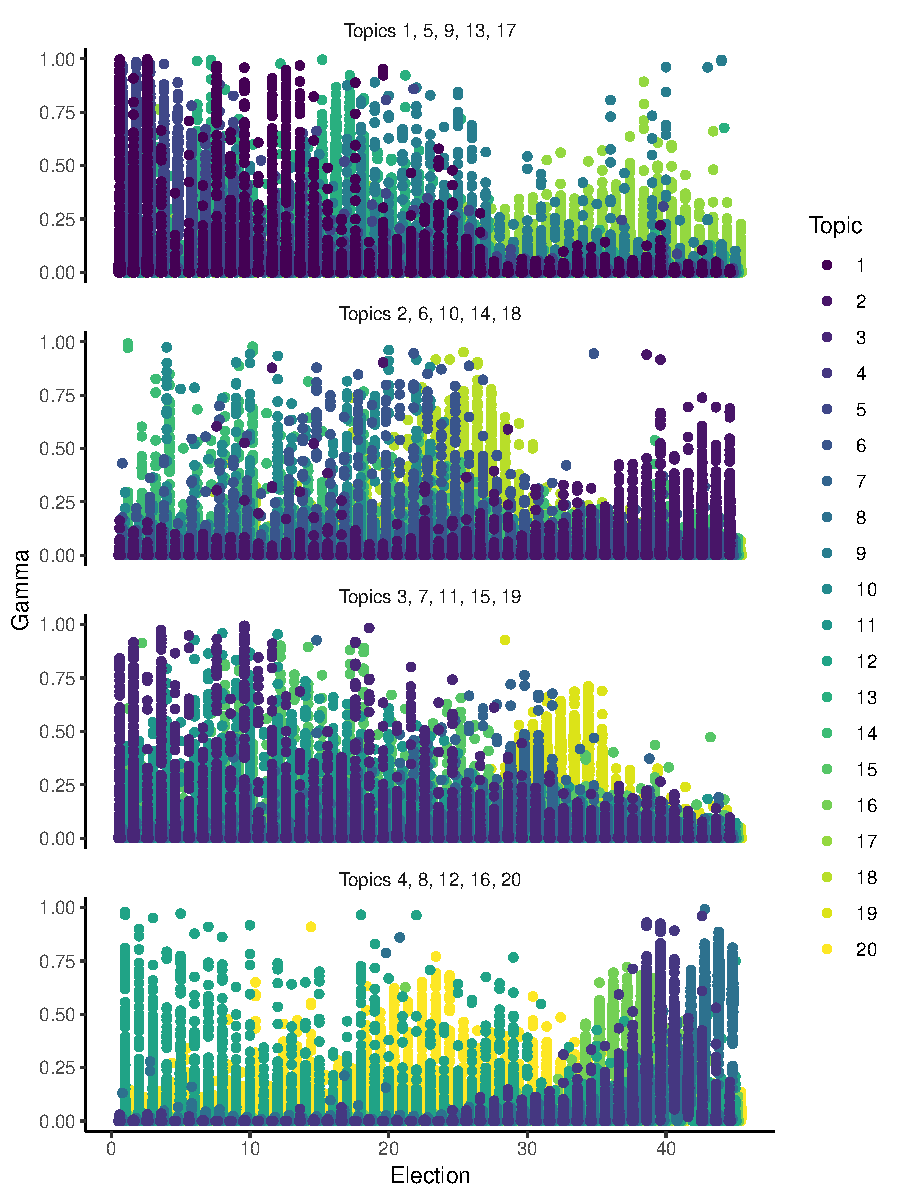
\includegraphics[width=1\linewidth]{/Users/rohanalexander/Documents/phd/hansard/outputs/figures/2018-09-28-topics_separated_by_election} \caption{Topic proportions grouped by elections}\label{fig:electionsevents}
\end{figure}

Figure \ref{fig:governmentevents} shows the grouping by government. This
can be different to election groupings, for instance, the change from
the Rudd to Gillard governments happened without an election. Similarly,
John Howard's three terms are all considered the one government for our
purposes.

Here we see much more difference between adjacent events. This suggests
that new governments tend to talk about different topics than the
government they replace.

\begin{figure}
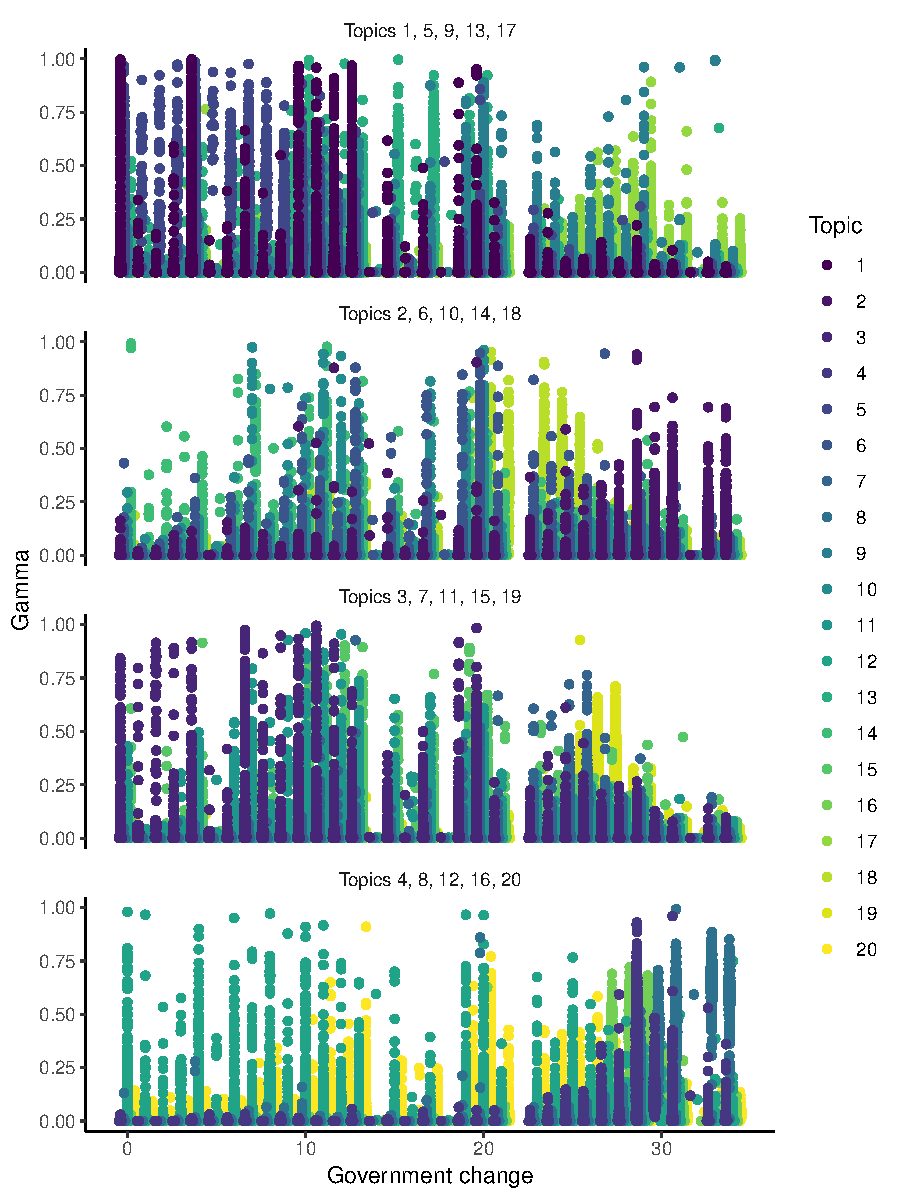
\includegraphics[width=1\linewidth]{/Users/rohanalexander/Documents/phd/hansard/outputs/figures/2018-09-28-topics_separated_by_government_change} \caption{Topic proportions grouped by government}\label{fig:governmentevents}
\end{figure}

Figure \ref{fig:economicevents} shows the grouping by major economic
changes. There are considerable changes between adjacent events.

\begin{figure}
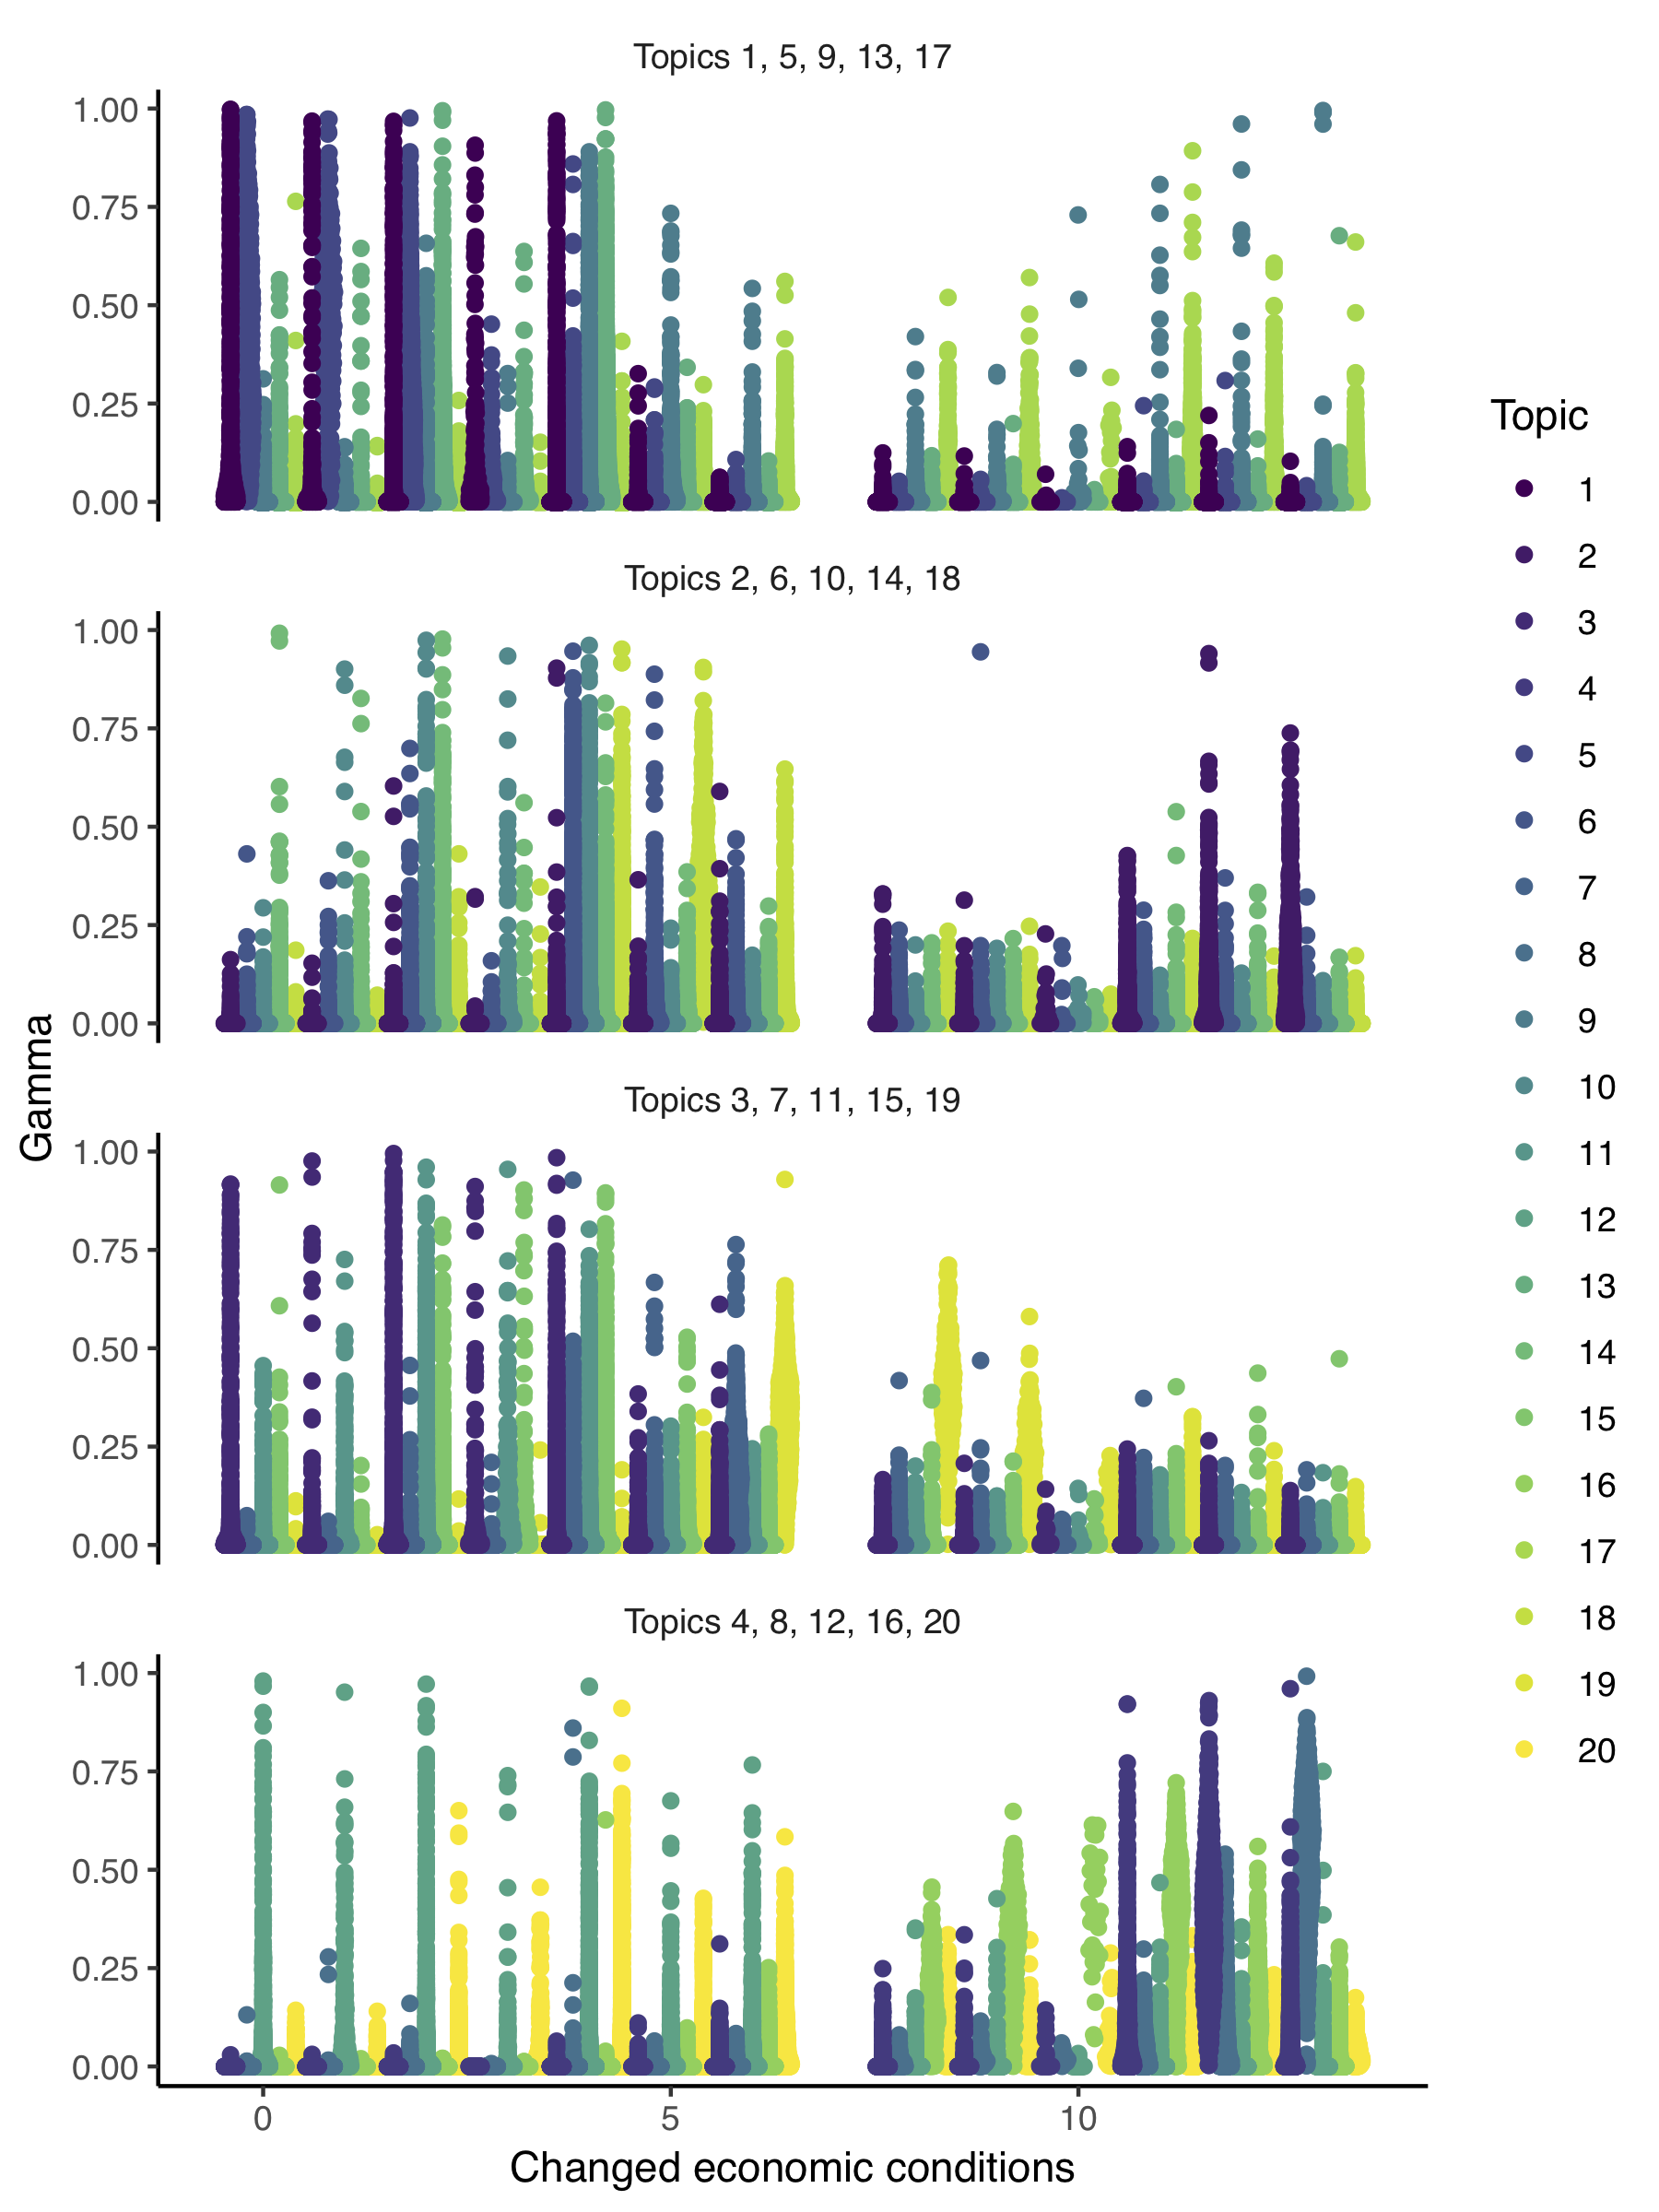
\includegraphics[width=1\linewidth]{/Users/rohanalexander/Documents/phd/hansard/outputs/figures/2018-09-28-topics_separated_by_economic_changes} \caption{Topic proportions grouped by economic events}\label{fig:economicevents}
\end{figure}

Figure \ref{fig:otherevents} shows the grouping by major other events,
such as the 9/11 attacks.

\begin{figure}
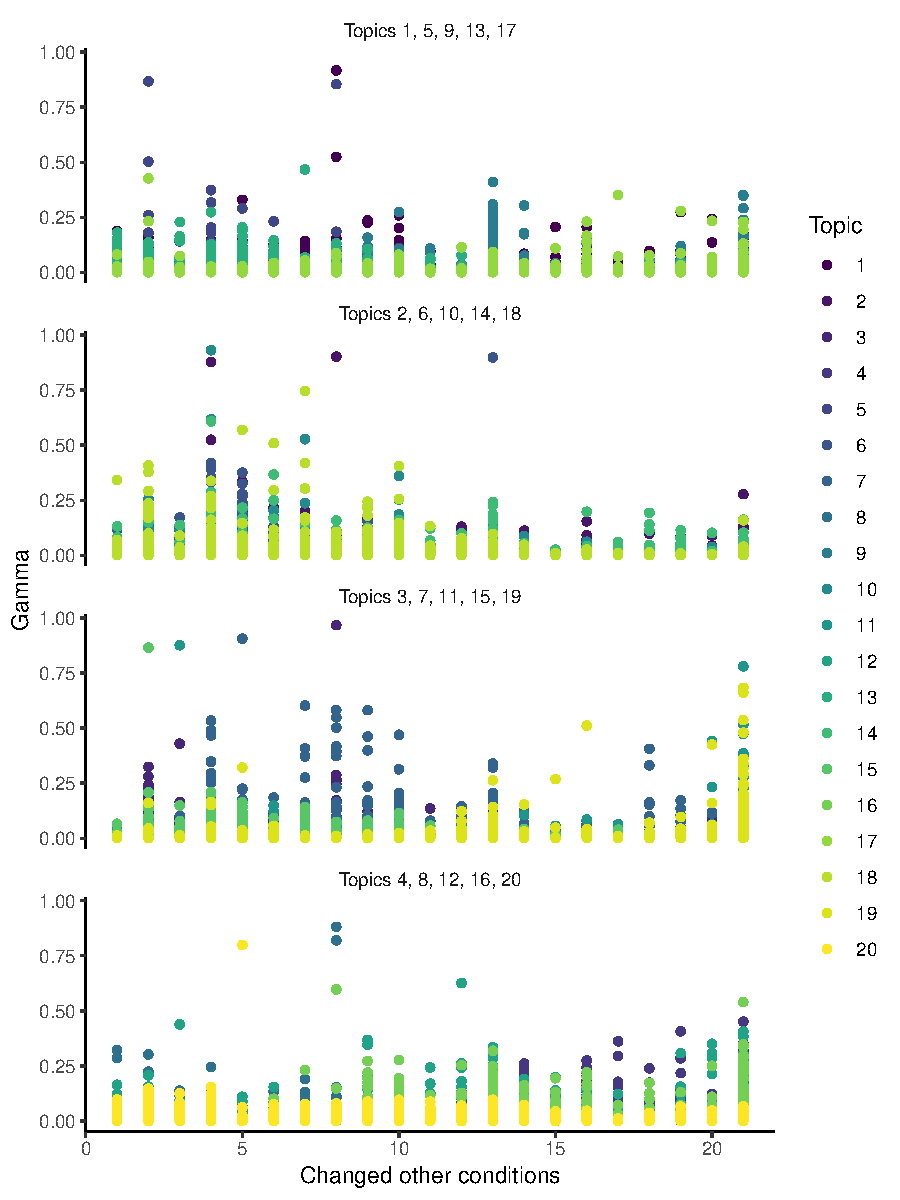
\includegraphics[width=1\linewidth]{/Users/rohanalexander/Documents/phd/hansard/outputs/figures/2018-09-28-topics_separated_by_other_changes} \caption{Topic proportions grouped by other events}\label{fig:otherevents}
\end{figure}

Another way to consider the effect of events is by including
incrementing variables in the prevelance metadata. This then gets
included in the topic modelling and the significance to each topic can
be computed. Table \ref{tab:dodgysignificances} summarises these by the
type of dummy and the topic. At the five per cent level the events that
we consider were significant for eight topics. This significance tended
to be correlated, especially for economic and other events.

\begin{table}

\caption{\label{tab:dodgysignificances}Significance of dummy}
\centering
\fontsize{12}{14}\selectfont
\begin{tabular}[t]{rrrrr}
\toprule
Topic & Elections & Governments & Economic & Other\\
\midrule
1 & 0.00 & 0.00 & 0.00 & 0.04\\
2 & 0.50 & 0.69 & 0.15 & 0.64\\
3 & 0.18 & 0.36 & 0.28 & 0.58\\
4 & 0.90 & 0.20 & 0.00 & 0.00\\
5 & 0.88 & 0.15 & 0.15 & 0.70\\
\addlinespace
6 & 0.41 & 0.00 & 0.21 & 0.20\\
7 & 0.03 & 0.00 & 0.00 & 0.00\\
8 & 0.61 & 0.39 & 0.00 & 0.00\\
9 & 0.18 & 0.24 & 0.83 & 0.62\\
10 & 0.99 & 0.34 & 0.96 & 0.41\\
\addlinespace
11 & 0.00 & 0.13 & 0.18 & 0.22\\
12 & 0.03 & 0.02 & 0.06 & 0.27\\
13 & 0.00 & 0.00 & 0.00 & 0.00\\
14 & 0.01 & 0.37 & 0.22 & 0.28\\
15 & 0.62 & 0.50 & 0.12 & 0.64\\
\addlinespace
16 & 0.74 & 0.00 & 0.00 & 0.00\\
17 & 0.01 & 0.40 & 0.80 & 0.16\\
18 & 0.23 & 0.00 & 0.00 & 0.00\\
19 & 0.31 & 0.00 & 0.00 & 0.00\\
20 & 0.00 & 0.54 & 0.09 & 0.35\\
\bottomrule
\end{tabular}
\end{table}

For instance, all of the incrementing variables have a significant
effect on the prevalence of Topic 1. Table \ref{tab:topwordssig} shows
that this has to do with tariffs and trade. On the other hand, Topic 2
has to do with aspects of daily life such as community and children, and
Topic 3 has to do with legal issues and neither is significant. This is
not surprising given the centrality of these concerns at all times.

\begin{table}

\caption{\label{tab:topwordssig}Top words for each topic}
\centering
\fontsize{12}{14}\selectfont
\begin{tabular}[t]{rl}
\toprule
Topic & Top words\\
\midrule
1 & tariff, duties, trade, customs, protection, item, industries\\
2 & community, life, children, family, australians, women, rights\\
3 & court, industrial, union, law, trade, arbitration, workers\\
4 & services, community, care, education, funding, health, school\\
5 & joseph, connection, money, federal, sydney, officers, service\\
\addlinespace
6 & pension, health, medical, scheme, service, week, social\\
7 & total, roads, wul, expenditure, road, budget, assistance\\
8 & health, billion, business, electorate, senator, community, budget\\
9 & united, world, nations, international, war, defence, foreign\\
10 & bank, royal, private, control, broadcasting, banking, money\\
\addlinespace
11 & taxation, income, treasurer, revenue, money, land, financial\\
12 & speaker, vote, motion, senate, election, standing, electoral\\
13 & war, defence, service, british, ill, britain, soldiers\\
14 & territory, oil, northern, line, shipping, ships, company\\
15 & wheat, wool, primary, production, farmers, export, zealand\\
\addlinespace
16 & tion, business, ing, governments, issue, speaker, health\\
17 & amendments, section, information, service, person, provisions, law\\
18 & education, service, development, housing, capital, territory, services\\
19 & speaker, deputy, petitioners, petition, ing, pray, citizens\\
20 & budget, economic, hear, employment, unemployment, governments, economy\\
\bottomrule
\end{tabular}
\end{table}

\section{Summary and conclusions}\label{summary-and-conclusions}

In this paper we examined what was said in Australia's parliaments. We
downloaded and parsed PDFs for Australian states and federal
parliaments. We then used a text model to group the discussions into
topics and analysed the effect of various events on the distribution of
the discussion.

In general we found that changes in government changed the distribution
of topics discussed in parliament, but that elections did not. We found
that significant events such as 9/11 had substantial and lasting
changes, but that with certain exceptions, economic events did not.

Text analysis has well-known biases and weaknesses and is a complement
to more detailed analysis such as qualitative methods and case studies.
We consider the results presented in this paper, as well as many of
those results of the larger text-as-data research program, as fitting
within findings based on other methods.

\newpage

\appendix


\section{Appendix}\label{appendix}

\subsection{Example page}\label{example-page}

Figure \ref{fig:asdf}

\begin{figure}
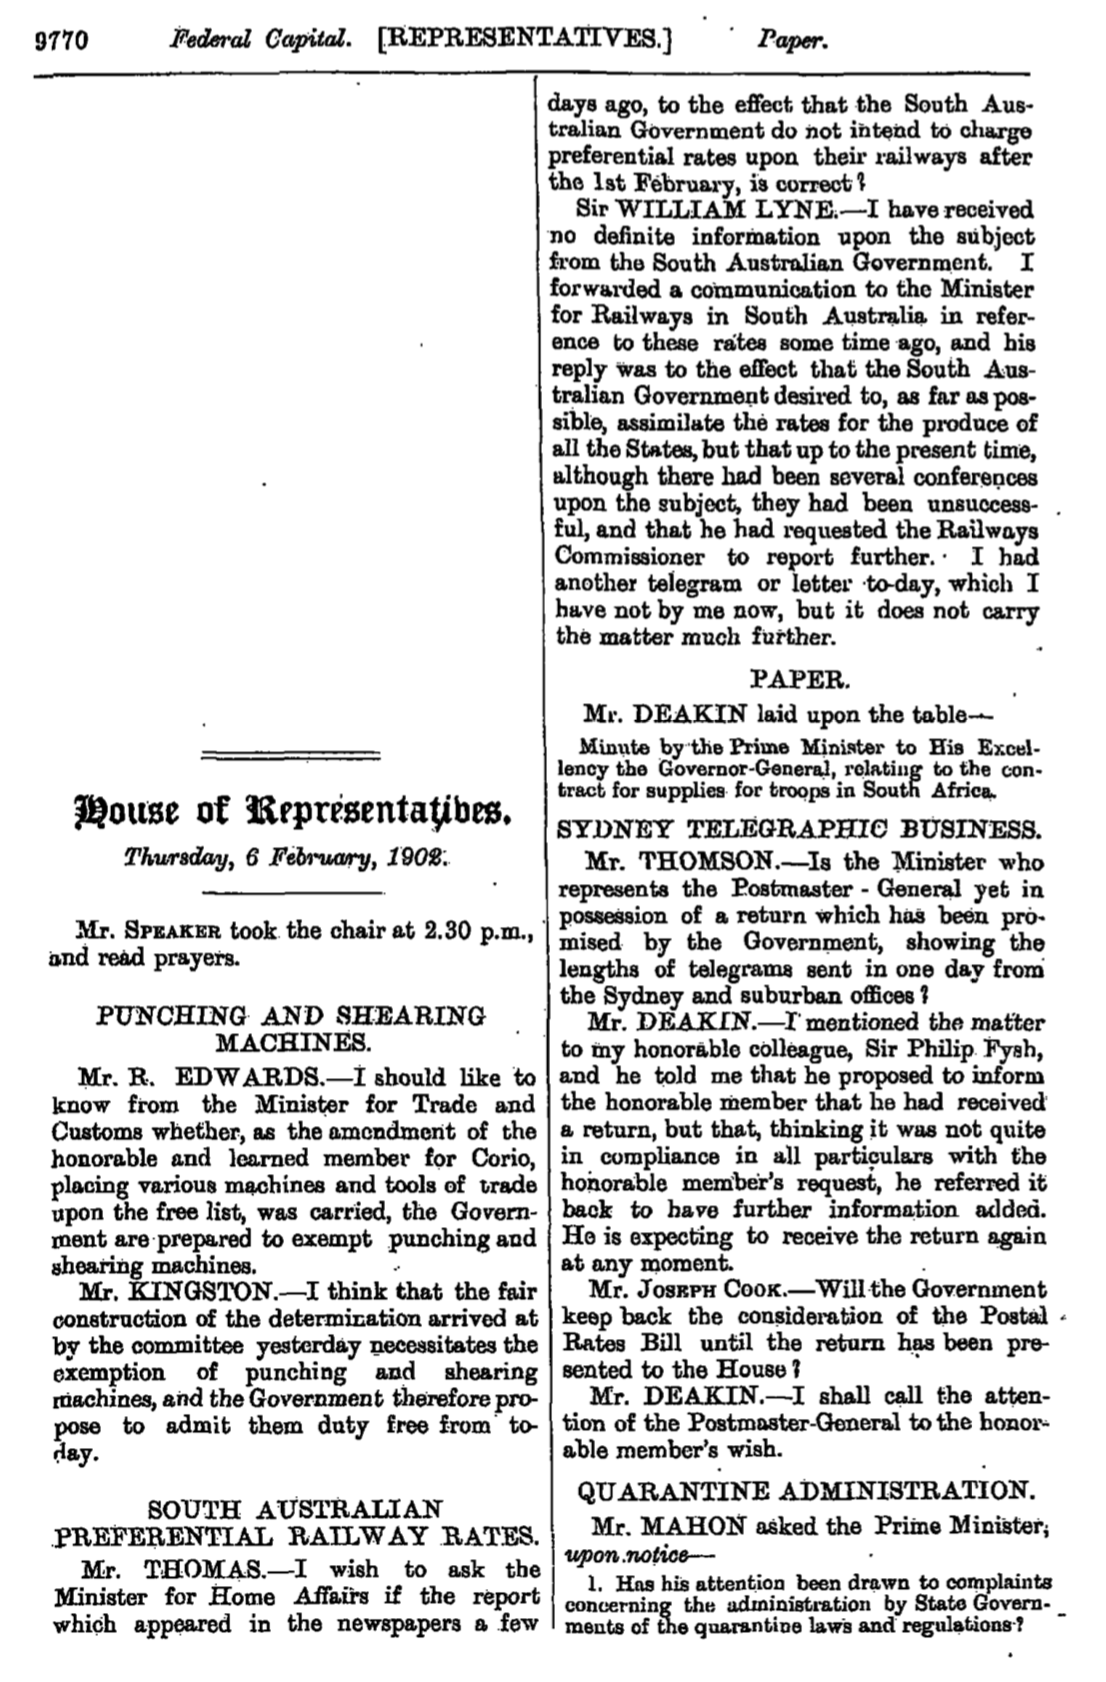
\includegraphics[width=1\linewidth]{/Users/rohanalexander/Documents/phd/hansard/outputs/figures/example_hansard_page} \caption{Example Hansard page - 6 February 1902}\label{fig:asdf}
\end{figure}

\subsection{Document sources}\label{document-sources}

Where from?

Which years are being used (not non-OCRd)

\subsection{Dataset issues}\label{dataset-issues}

Which PDFs are missing or have no content, etc.

\begin{longtable}[]{@{}lllllll@{}}
\toprule
\begin{minipage}[b]{0.02\columnwidth}\raggedright\strut
year\strut
\end{minipage} & \begin{minipage}[b]{0.09\columnwidth}\raggedright\strut
I have this number in Reps\strut
\end{minipage} & \begin{minipage}[b]{0.10\columnwidth}\raggedright\strut
They say this number in Senate\strut
\end{minipage} & \begin{minipage}[b]{0.10\columnwidth}\raggedright\strut
They say this number in Reps\strut
\end{minipage} & \begin{minipage}[b]{0.07\columnwidth}\raggedright\strut
Difference in Reps\strut
\end{minipage} & \begin{minipage}[b]{0.11\columnwidth}\raggedright\strut
Comment\strut
\end{minipage} & \begin{minipage}[b]{0.31\columnwidth}\raggedright\strut
Source\strut
\end{minipage}\tabularnewline
\midrule
\endhead
\begin{minipage}[t]{0.02\columnwidth}\raggedright\strut
1902\strut
\end{minipage} & \begin{minipage}[t]{0.09\columnwidth}\raggedright\strut
106\strut
\end{minipage} & \begin{minipage}[t]{0.10\columnwidth}\raggedright\strut
93\strut
\end{minipage} & \begin{minipage}[t]{0.10\columnwidth}\raggedright\strut
107\strut
\end{minipage} & \begin{minipage}[t]{0.07\columnwidth}\raggedright\strut
1\strut
\end{minipage} & \begin{minipage}[t]{0.11\columnwidth}\raggedright\strut
Positive means I am missing some\strut
\end{minipage} & \begin{minipage}[t]{0.31\columnwidth}\raggedright\strut
\url{https://www.aph.gov.au/Parliamentary_Business/Statistics/Senate_StatsNet/General/sittingdaysyear}\strut
\end{minipage}\tabularnewline
\begin{minipage}[t]{0.02\columnwidth}\raggedright\strut
1908\strut
\end{minipage} & \begin{minipage}[t]{0.09\columnwidth}\raggedright\strut
93\strut
\end{minipage} & \begin{minipage}[t]{0.10\columnwidth}\raggedright\strut
84\strut
\end{minipage} & \begin{minipage}[t]{0.10\columnwidth}\raggedright\strut
91\strut
\end{minipage} & \begin{minipage}[t]{0.07\columnwidth}\raggedright\strut
-2\strut
\end{minipage} & \begin{minipage}[t]{0.11\columnwidth}\raggedright\strut
Negative means I have too many\strut
\end{minipage} & \begin{minipage}[t]{0.31\columnwidth}\raggedright\strut
\strut
\end{minipage}\tabularnewline
\begin{minipage}[t]{0.02\columnwidth}\raggedright\strut
1909\strut
\end{minipage} & \begin{minipage}[t]{0.09\columnwidth}\raggedright\strut
97\strut
\end{minipage} & \begin{minipage}[t]{0.10\columnwidth}\raggedright\strut
71\strut
\end{minipage} & \begin{minipage}[t]{0.10\columnwidth}\raggedright\strut
98\strut
\end{minipage} & \begin{minipage}[t]{0.07\columnwidth}\raggedright\strut
1\strut
\end{minipage} & \begin{minipage}[t]{0.11\columnwidth}\raggedright\strut
\strut
\end{minipage} & \begin{minipage}[t]{0.31\columnwidth}\raggedright\strut
\strut
\end{minipage}\tabularnewline
\begin{minipage}[t]{0.02\columnwidth}\raggedright\strut
1918\strut
\end{minipage} & \begin{minipage}[t]{0.09\columnwidth}\raggedright\strut
87\strut
\end{minipage} & \begin{minipage}[t]{0.10\columnwidth}\raggedright\strut
68\strut
\end{minipage} & \begin{minipage}[t]{0.10\columnwidth}\raggedright\strut
86\strut
\end{minipage} & \begin{minipage}[t]{0.07\columnwidth}\raggedright\strut
-1\strut
\end{minipage} & \begin{minipage}[t]{0.11\columnwidth}\raggedright\strut
\strut
\end{minipage} & \begin{minipage}[t]{0.31\columnwidth}\raggedright\strut
\strut
\end{minipage}\tabularnewline
\begin{minipage}[t]{0.02\columnwidth}\raggedright\strut
1920\strut
\end{minipage} & \begin{minipage}[t]{0.09\columnwidth}\raggedright\strut
113\strut
\end{minipage} & \begin{minipage}[t]{0.10\columnwidth}\raggedright\strut
76\strut
\end{minipage} & \begin{minipage}[t]{0.10\columnwidth}\raggedright\strut
114\strut
\end{minipage} & \begin{minipage}[t]{0.07\columnwidth}\raggedright\strut
1\strut
\end{minipage} & \begin{minipage}[t]{0.11\columnwidth}\raggedright\strut
\strut
\end{minipage} & \begin{minipage}[t]{0.31\columnwidth}\raggedright\strut
\strut
\end{minipage}\tabularnewline
\begin{minipage}[t]{0.02\columnwidth}\raggedright\strut
1921\strut
\end{minipage} & \begin{minipage}[t]{0.09\columnwidth}\raggedright\strut
92\strut
\end{minipage} & \begin{minipage}[t]{0.10\columnwidth}\raggedright\strut
79\strut
\end{minipage} & \begin{minipage}[t]{0.10\columnwidth}\raggedright\strut
93\strut
\end{minipage} & \begin{minipage}[t]{0.07\columnwidth}\raggedright\strut
1\strut
\end{minipage} & \begin{minipage}[t]{0.11\columnwidth}\raggedright\strut
\strut
\end{minipage} & \begin{minipage}[t]{0.31\columnwidth}\raggedright\strut
\strut
\end{minipage}\tabularnewline
\begin{minipage}[t]{0.02\columnwidth}\raggedright\strut
1934\strut
\end{minipage} & \begin{minipage}[t]{0.09\columnwidth}\raggedright\strut
36\strut
\end{minipage} & \begin{minipage}[t]{0.10\columnwidth}\raggedright\strut
22\strut
\end{minipage} & \begin{minipage}[t]{0.10\columnwidth}\raggedright\strut
35\strut
\end{minipage} & \begin{minipage}[t]{0.07\columnwidth}\raggedright\strut
-1\strut
\end{minipage} & \begin{minipage}[t]{0.11\columnwidth}\raggedright\strut
\strut
\end{minipage} & \begin{minipage}[t]{0.31\columnwidth}\raggedright\strut
\strut
\end{minipage}\tabularnewline
\begin{minipage}[t]{0.02\columnwidth}\raggedright\strut
1935\strut
\end{minipage} & \begin{minipage}[t]{0.09\columnwidth}\raggedright\strut
54\strut
\end{minipage} & \begin{minipage}[t]{0.10\columnwidth}\raggedright\strut
37\strut
\end{minipage} & \begin{minipage}[t]{0.10\columnwidth}\raggedright\strut
55\strut
\end{minipage} & \begin{minipage}[t]{0.07\columnwidth}\raggedright\strut
1\strut
\end{minipage} & \begin{minipage}[t]{0.11\columnwidth}\raggedright\strut
\strut
\end{minipage} & \begin{minipage}[t]{0.31\columnwidth}\raggedright\strut
\strut
\end{minipage}\tabularnewline
\begin{minipage}[t]{0.02\columnwidth}\raggedright\strut
1942\strut
\end{minipage} & \begin{minipage}[t]{0.09\columnwidth}\raggedright\strut
44\strut
\end{minipage} & \begin{minipage}[t]{0.10\columnwidth}\raggedright\strut
36\strut
\end{minipage} & \begin{minipage}[t]{0.10\columnwidth}\raggedright\strut
45\strut
\end{minipage} & \begin{minipage}[t]{0.07\columnwidth}\raggedright\strut
1\strut
\end{minipage} & \begin{minipage}[t]{0.11\columnwidth}\raggedright\strut
\strut
\end{minipage} & \begin{minipage}[t]{0.31\columnwidth}\raggedright\strut
\strut
\end{minipage}\tabularnewline
\begin{minipage}[t]{0.02\columnwidth}\raggedright\strut
1948\strut
\end{minipage} & \begin{minipage}[t]{0.09\columnwidth}\raggedright\strut
89\strut
\end{minipage} & \begin{minipage}[t]{0.10\columnwidth}\raggedright\strut
39\strut
\end{minipage} & \begin{minipage}[t]{0.10\columnwidth}\raggedright\strut
90\strut
\end{minipage} & \begin{minipage}[t]{0.07\columnwidth}\raggedright\strut
1\strut
\end{minipage} & \begin{minipage}[t]{0.11\columnwidth}\raggedright\strut
\strut
\end{minipage} & \begin{minipage}[t]{0.31\columnwidth}\raggedright\strut
\strut
\end{minipage}\tabularnewline
\begin{minipage}[t]{0.02\columnwidth}\raggedright\strut
1951\strut
\end{minipage} & \begin{minipage}[t]{0.09\columnwidth}\raggedright\strut
55\strut
\end{minipage} & \begin{minipage}[t]{0.10\columnwidth}\raggedright\strut
40\strut
\end{minipage} & \begin{minipage}[t]{0.10\columnwidth}\raggedright\strut
56\strut
\end{minipage} & \begin{minipage}[t]{0.07\columnwidth}\raggedright\strut
1\strut
\end{minipage} & \begin{minipage}[t]{0.11\columnwidth}\raggedright\strut
\strut
\end{minipage} & \begin{minipage}[t]{0.31\columnwidth}\raggedright\strut
\strut
\end{minipage}\tabularnewline
\begin{minipage}[t]{0.02\columnwidth}\raggedright\strut
1955\strut
\end{minipage} & \begin{minipage}[t]{0.09\columnwidth}\raggedright\strut
53\strut
\end{minipage} & \begin{minipage}[t]{0.10\columnwidth}\raggedright\strut
36\strut
\end{minipage} & \begin{minipage}[t]{0.10\columnwidth}\raggedright\strut
52\strut
\end{minipage} & \begin{minipage}[t]{0.07\columnwidth}\raggedright\strut
-1\strut
\end{minipage} & \begin{minipage}[t]{0.11\columnwidth}\raggedright\strut
\strut
\end{minipage} & \begin{minipage}[t]{0.31\columnwidth}\raggedright\strut
\strut
\end{minipage}\tabularnewline
\begin{minipage}[t]{0.02\columnwidth}\raggedright\strut
1974\strut
\end{minipage} & \begin{minipage}[t]{0.09\columnwidth}\raggedright\strut
64\strut
\end{minipage} & \begin{minipage}[t]{0.10\columnwidth}\raggedright\strut
64\strut
\end{minipage} & \begin{minipage}[t]{0.10\columnwidth}\raggedright\strut
62\strut
\end{minipage} & \begin{minipage}[t]{0.07\columnwidth}\raggedright\strut
-2\strut
\end{minipage} & \begin{minipage}[t]{0.11\columnwidth}\raggedright\strut
\strut
\end{minipage} & \begin{minipage}[t]{0.31\columnwidth}\raggedright\strut
\strut
\end{minipage}\tabularnewline
\begin{minipage}[t]{0.02\columnwidth}\raggedright\strut
1985\strut
\end{minipage} & \begin{minipage}[t]{0.09\columnwidth}\raggedright\strut
65\strut
\end{minipage} & \begin{minipage}[t]{0.10\columnwidth}\raggedright\strut
74\strut
\end{minipage} & \begin{minipage}[t]{0.10\columnwidth}\raggedright\strut
66\strut
\end{minipage} & \begin{minipage}[t]{0.07\columnwidth}\raggedright\strut
1\strut
\end{minipage} & \begin{minipage}[t]{0.11\columnwidth}\raggedright\strut
\strut
\end{minipage} & \begin{minipage}[t]{0.31\columnwidth}\raggedright\strut
\strut
\end{minipage}\tabularnewline
\begin{minipage}[t]{0.02\columnwidth}\raggedright\strut
1991\strut
\end{minipage} & \begin{minipage}[t]{0.09\columnwidth}\raggedright\strut
66\strut
\end{minipage} & \begin{minipage}[t]{0.10\columnwidth}\raggedright\strut
83\strut
\end{minipage} & \begin{minipage}[t]{0.10\columnwidth}\raggedright\strut
67\strut
\end{minipage} & \begin{minipage}[t]{0.07\columnwidth}\raggedright\strut
1\strut
\end{minipage} & \begin{minipage}[t]{0.11\columnwidth}\raggedright\strut
\strut
\end{minipage} & \begin{minipage}[t]{0.31\columnwidth}\raggedright\strut
\strut
\end{minipage}\tabularnewline
\begin{minipage}[t]{0.02\columnwidth}\raggedright\strut
1992\strut
\end{minipage} & \begin{minipage}[t]{0.09\columnwidth}\raggedright\strut
60\strut
\end{minipage} & \begin{minipage}[t]{0.10\columnwidth}\raggedright\strut
76\strut
\end{minipage} & \begin{minipage}[t]{0.10\columnwidth}\raggedright\strut
44\strut
\end{minipage} & \begin{minipage}[t]{0.07\columnwidth}\raggedright\strut
-16\strut
\end{minipage} & \begin{minipage}[t]{0.11\columnwidth}\raggedright\strut
\strut
\end{minipage} & \begin{minipage}[t]{0.31\columnwidth}\raggedright\strut
\strut
\end{minipage}\tabularnewline
\begin{minipage}[t]{0.02\columnwidth}\raggedright\strut
1993\strut
\end{minipage} & \begin{minipage}[t]{0.09\columnwidth}\raggedright\strut
47\strut
\end{minipage} & \begin{minipage}[t]{0.10\columnwidth}\raggedright\strut
53\strut
\end{minipage} & \begin{minipage}[t]{0.10\columnwidth}\raggedright\strut
46\strut
\end{minipage} & \begin{minipage}[t]{0.07\columnwidth}\raggedright\strut
-1\strut
\end{minipage} & \begin{minipage}[t]{0.11\columnwidth}\raggedright\strut
\strut
\end{minipage} & \begin{minipage}[t]{0.31\columnwidth}\raggedright\strut
\strut
\end{minipage}\tabularnewline
\begin{minipage}[t]{0.02\columnwidth}\raggedright\strut
1994\strut
\end{minipage} & \begin{minipage}[t]{0.09\columnwidth}\raggedright\strut
69\strut
\end{minipage} & \begin{minipage}[t]{0.10\columnwidth}\raggedright\strut
80\strut
\end{minipage} & \begin{minipage}[t]{0.10\columnwidth}\raggedright\strut
68\strut
\end{minipage} & \begin{minipage}[t]{0.07\columnwidth}\raggedright\strut
-1\strut
\end{minipage} & \begin{minipage}[t]{0.11\columnwidth}\raggedright\strut
\strut
\end{minipage} & \begin{minipage}[t]{0.31\columnwidth}\raggedright\strut
\strut
\end{minipage}\tabularnewline
\begin{minipage}[t]{0.02\columnwidth}\raggedright\strut
1995\strut
\end{minipage} & \begin{minipage}[t]{0.09\columnwidth}\raggedright\strut
71\strut
\end{minipage} & \begin{minipage}[t]{0.10\columnwidth}\raggedright\strut
78\strut
\end{minipage} & \begin{minipage}[t]{0.10\columnwidth}\raggedright\strut
70\strut
\end{minipage} & \begin{minipage}[t]{0.07\columnwidth}\raggedright\strut
-1\strut
\end{minipage} & \begin{minipage}[t]{0.11\columnwidth}\raggedright\strut
\strut
\end{minipage} & \begin{minipage}[t]{0.31\columnwidth}\raggedright\strut
\strut
\end{minipage}\tabularnewline
\begin{minipage}[t]{0.02\columnwidth}\raggedright\strut
1997\strut
\end{minipage} & \begin{minipage}[t]{0.09\columnwidth}\raggedright\strut
79\strut
\end{minipage} & \begin{minipage}[t]{0.10\columnwidth}\raggedright\strut
82\strut
\end{minipage} & \begin{minipage}[t]{0.10\columnwidth}\raggedright\strut
76\strut
\end{minipage} & \begin{minipage}[t]{0.07\columnwidth}\raggedright\strut
-3\strut
\end{minipage} & \begin{minipage}[t]{0.11\columnwidth}\raggedright\strut
\strut
\end{minipage} & \begin{minipage}[t]{0.31\columnwidth}\raggedright\strut
\strut
\end{minipage}\tabularnewline
\begin{minipage}[t]{0.02\columnwidth}\raggedright\strut
1998\strut
\end{minipage} & \begin{minipage}[t]{0.09\columnwidth}\raggedright\strut
56\strut
\end{minipage} & \begin{minipage}[t]{0.10\columnwidth}\raggedright\strut
57\strut
\end{minipage} & \begin{minipage}[t]{0.10\columnwidth}\raggedright\strut
54\strut
\end{minipage} & \begin{minipage}[t]{0.07\columnwidth}\raggedright\strut
-2\strut
\end{minipage} & \begin{minipage}[t]{0.11\columnwidth}\raggedright\strut
\strut
\end{minipage} & \begin{minipage}[t]{0.31\columnwidth}\raggedright\strut
\strut
\end{minipage}\tabularnewline
\begin{minipage}[t]{0.02\columnwidth}\raggedright\strut
2000\strut
\end{minipage} & \begin{minipage}[t]{0.09\columnwidth}\raggedright\strut
71\strut
\end{minipage} & \begin{minipage}[t]{0.10\columnwidth}\raggedright\strut
71\strut
\end{minipage} & \begin{minipage}[t]{0.10\columnwidth}\raggedright\strut
73\strut
\end{minipage} & \begin{minipage}[t]{0.07\columnwidth}\raggedright\strut
2\strut
\end{minipage} & \begin{minipage}[t]{0.11\columnwidth}\raggedright\strut
\strut
\end{minipage} & \begin{minipage}[t]{0.31\columnwidth}\raggedright\strut
\strut
\end{minipage}\tabularnewline
\begin{minipage}[t]{0.02\columnwidth}\raggedright\strut
2002\strut
\end{minipage} & \begin{minipage}[t]{0.09\columnwidth}\raggedright\strut
68\strut
\end{minipage} & \begin{minipage}[t]{0.10\columnwidth}\raggedright\strut
60\strut
\end{minipage} & \begin{minipage}[t]{0.10\columnwidth}\raggedright\strut
69\strut
\end{minipage} & \begin{minipage}[t]{0.07\columnwidth}\raggedright\strut
1\strut
\end{minipage} & \begin{minipage}[t]{0.11\columnwidth}\raggedright\strut
\strut
\end{minipage} & \begin{minipage}[t]{0.31\columnwidth}\raggedright\strut
\strut
\end{minipage}\tabularnewline
\begin{minipage}[t]{0.02\columnwidth}\raggedright\strut
2003\strut
\end{minipage} & \begin{minipage}[t]{0.09\columnwidth}\raggedright\strut
74\strut
\end{minipage} & \begin{minipage}[t]{0.10\columnwidth}\raggedright\strut
64\strut
\end{minipage} & \begin{minipage}[t]{0.10\columnwidth}\raggedright\strut
75\strut
\end{minipage} & \begin{minipage}[t]{0.07\columnwidth}\raggedright\strut
1\strut
\end{minipage} & \begin{minipage}[t]{0.11\columnwidth}\raggedright\strut
\strut
\end{minipage} & \begin{minipage}[t]{0.31\columnwidth}\raggedright\strut
\strut
\end{minipage}\tabularnewline
\begin{minipage}[t]{0.02\columnwidth}\raggedright\strut
2004\strut
\end{minipage} & \begin{minipage}[t]{0.09\columnwidth}\raggedright\strut
58\strut
\end{minipage} & \begin{minipage}[t]{0.10\columnwidth}\raggedright\strut
49\strut
\end{minipage} & \begin{minipage}[t]{0.10\columnwidth}\raggedright\strut
59\strut
\end{minipage} & \begin{minipage}[t]{0.07\columnwidth}\raggedright\strut
1\strut
\end{minipage} & \begin{minipage}[t]{0.11\columnwidth}\raggedright\strut
\strut
\end{minipage} & \begin{minipage}[t]{0.31\columnwidth}\raggedright\strut
\strut
\end{minipage}\tabularnewline
\begin{minipage}[t]{0.02\columnwidth}\raggedright\strut
2012\strut
\end{minipage} & \begin{minipage}[t]{0.09\columnwidth}\raggedright\strut
63\strut
\end{minipage} & \begin{minipage}[t]{0.10\columnwidth}\raggedright\strut
57\strut
\end{minipage} & \begin{minipage}[t]{0.10\columnwidth}\raggedright\strut
67\strut
\end{minipage} & \begin{minipage}[t]{0.07\columnwidth}\raggedright\strut
4\strut
\end{minipage} & \begin{minipage}[t]{0.11\columnwidth}\raggedright\strut
\strut
\end{minipage} & \begin{minipage}[t]{0.31\columnwidth}\raggedright\strut
\strut
\end{minipage}\tabularnewline
\bottomrule
\end{longtable}

\subsection{Example workflow}\label{example-workflow}

Example of the workflow from PDF to text

\subsection{PDF to CSV issues}\label{pdf-to-csv-issues}

Insert graph of stop words over time.

\subsection{Topic modelling example and
details}\label{topic-modelling-example-and-details}

\subsubsection{Examples}\label{examples}

For instance, if there were five topics and two documents, then the
first document may be comprised mostly of the first few topics; the
other document may be mostly about the final few topics (Figure
\ref{fig:topicsoverdocuments}).

\begin{figure}
\centering
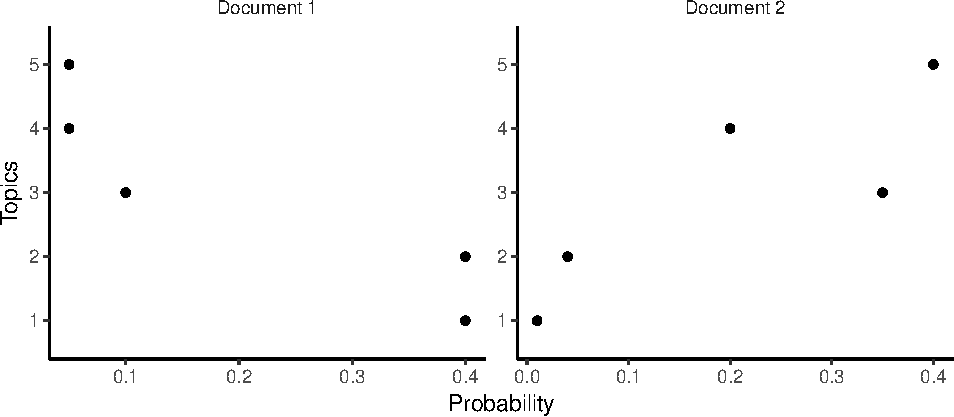
\includegraphics{svm-rmarkdown-article-example_files/figure-latex/topicsoverdocuments-1.pdf}
\caption{\label{fig:topicsoverdocuments}Probability distributions over
topics for two documents}
\end{figure}

For instance, if there were ten terms, then one topic could be defined
by giving more weight to terms related to immigration; and some other
topic may give more weight to terms related to the economy (Figure
\ref{fig:topicsoverterms}).

\begin{figure}
\centering
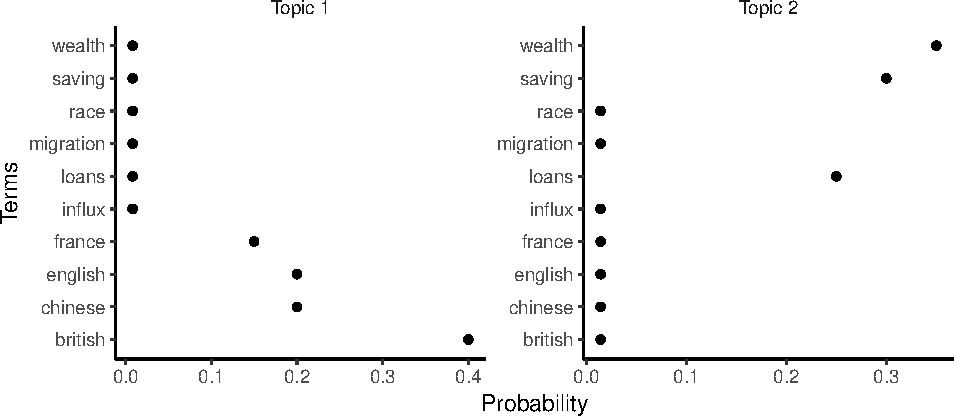
\includegraphics{svm-rmarkdown-article-example_files/figure-latex/topicsoverterms-1.pdf}
\caption{\label{fig:topicsoverterms}Probability distributions over terms}
\end{figure}

\subsubsection{Solution details}\label{solution-details}

Following \citet{SteyversGriffiths2006} and \citet{Darling2011}, the
Gibbs sampling process attempts to find a topic for a particular term in
a particular document, given the topics of all other terms for all other
documents. Broadly, it does this by first assigning every term in every
document to a random topic, specified by Dirichlet priors with
\(\alpha = \frac{50}{K}\) and \(\eta = 0.1\)
(\citet{SteyversGriffiths2006} recommends \(\eta = 0.01\)), where
\(\alpha\) refers to the distribution over topics and \(\eta\) refers to
the distribution over terms (\citet{Grun2011}, p.~7). It then selects a
particular term in a particular document and assigns it to a new topic
based on the conditional distribution where the topics for all other
terms in all documents are taken as given (\citet{Grun2011}, p.~6):
\[p(z_{d, n}=k | w_{1:D, 1:N}, z'_{d, n}) \propto \frac{\lambda'_{n\rightarrow k}+\eta}{\lambda'_{.\rightarrow k}+V\eta} \frac{\lambda'^{(d)}_{n\rightarrow k}+\alpha}{\lambda'^{(d)}_{-i}+K\alpha} \]
where \(z'_{d, n}\) refers to all other topic assignments;
\(\lambda'_{n\rightarrow k}\) is a count of how many other times that
term has been assigned to topic \(k\); \(\lambda'_{.\rightarrow k}\) is
a count of how many other times that any term has been assigned to topic
\(k\); \(\lambda'^{(d)}_{n\rightarrow k}\) is a count of how many other
times that term has been assigned to topic \(k\) in that particular
document; and \(\lambda'^{(d)}_{-i}\) is a count of how many other times
that term has been assigned in that document. Once \(z_{d,n}\) has been
estimated, then estimates for the distribution of words into topics and
topics into documents can be backed out.

This conditional distribution assigns topics depending on how often a
term has been assigned to that topic previously, and how common the
topic is in that document (\citet{SteyversGriffiths2006}). The initial
random allocation of topics means that the results of early passes
through the corpus of document are poor, but given enough time the
algorithm converges to an appropriate estimate.

\subsection{Selection of number of
topics}\label{selection-of-number-of-topics}

\subsection{Robustness of results}\label{robustness-of-results}

Here we change the number of sitting days considered either side of an
event. The results in the main section of the paper are for the nearest
ten days either side of an event. Here are show that the results are
essentially the same if the nearest one, two, five, and twenty days
either side of an event.

\subsection{Events}\label{events}

\begin{table}

\caption{\label{tab:governments}Change in governments}
\centering
\fontsize{8}{10}\selectfont
\begin{tabular}[t]{llllll}
\toprule
government & primeMinister & party & start & end & diedInOffice\\
\midrule
Barton & Edmund Barton & Protectionist & 1901-01-01 & 1903-09-24 & No\\
Deakin 1 & Alfred Deakin & Protectionist & 1903-09-24 & 1904-04-27 & No\\
Watson & Chris Watson & Labour & 1904-04-27 & 1904-08-18 & No\\
Reid & George Reid & Free Trade & 1904-08-18 & 1905-07-05 & No\\
Deakin 2 & Alfred Deakin & Protectionist & 1905-07-05 & 1908-11-13 & No\\
\addlinespace
Fisher 1 & Andrew Fisher & Labour & 1908-11-13 & 1909-06-02 & No\\
Deakin 3 & Alfred Deakin & Commonwealth Liberal & 1909-06-02 & 1910-04-29 & No\\
Fisher 2 & Andrew Fisher & Labor & 1910-04-29 & 1913-06-24 & No\\
Cook & Joseph Cook & Commonwealth Liberal & 1913-06-24 & 1914-09-17 & No\\
Fisher 3 & Andrew Fisher & Labor & 1914-09-17 & 1915-10-27 & No\\
\addlinespace
Hughes & Billy Hughes & Labor, National Labor and Nationalist & 1915-10-27 & 1923-02-09 & No\\
Bruce & Stanley Bruce & Nationalist (Coalition) & 1923-02-09 & 1929-10-22 & No\\
Scullin & James Scullin & Labor & 1929-10-22 & 1932-01-06 & No\\
Lyons & Joseph Lyons & United Australia (Coalition) & 1932-01-06 & 1939-04-07 & Yes\\
Page & Earle Page & Country (Coalition) & 1939-04-07 & 1939-04-26 & No\\
\addlinespace
Menzies 1 & Robert Menzies & United Australia (Coalition) & 1939-04-26 & 1941-08-28 & No\\
Fadden & Arthur Fadden & Country (Coalition) & 1941-08-28 & 1941-10-07 & No\\
Curtin & John Curtin & Labor & 1941-10-07 & 1945-07-05 & Yes\\
Forde & Frank Forde & Labor & 1945-07-06 & 1945-07-13 & No\\
Chifley & Ben Chifley & Labor & 1945-07-13 & 1949-12-19 & No\\
\addlinespace
Menzies 2 & Robert Menzies & Liberal (Coalition) & 1949-12-19 & 1966-01-26 & No\\
Holt & Harold Holt & Liberal (Coalition) & 1966-01-26 & 1967-12-19 & Yes\\
McEwen & John McEwen & Country (Coalition) & 1967-12-19 & 1968-01-10 & No\\
Gorton & John Gorton & Liberal (Coalition) & 1968-01-10 & 1971-03-10 & No\\
McMahon & William McMahon & Liberal (Coalition) & 1971-03-10 & 1972-12-05 & No\\
\addlinespace
Whitlam & Gough Whitlam & Labor & 1972-12-05 & 1975-11-11 & No\\
Fraser & Malcolm Fraser & Liberal (Coalition) & 1975-11-11 & 1983-03-11 & No\\
Hawke & Bob Hawke & Labor & 1983-03-11 & 1991-12-20 & No\\
Keating & Paul Keating & Labor & 1991-12-20 & 1996-03-11 & No\\
Howard & John Howard & Liberal (Coalition) & 1996-03-11 & 2007-12-03 & No\\
\addlinespace
Rudd 1 & Kevin Rudd & Labor & 2007-12-03 & 2010-06-24 & No\\
Gillard & Julia Gillard & Labor & 2010-06-24 & 2013-06-27 & No\\
Rudd 2 & Kevin Rudd & Labor & 2013-06-27 & 2013-09-18 & No\\
Abbott & Tony Abbott & Liberal (Coalition) & 2013-09-18 & 2015-09-15 & No\\
Turnbull & Malcolm Turnbull & Liberal (Coalition) & 2015-09-15 & 2018-08-24 & No\\
Morrison & Scott Morrison & Liberal (Coalition) & 2018-08-24 & NA & NA\\
\bottomrule
\end{tabular}
\end{table}

\begin{table}

\caption{\label{tab:elections}Elections}
\centering
\fontsize{8}{10}\selectfont
\begin{tabular}[t]{rll}
\toprule
year & electionDate & electionWinner\\
\midrule
1901 & 1901-03-29 & Non-labor\\
1903 & 1903-12-16 & Non-labor\\
1906 & 1906-12-12 & Non-labor\\
1910 & 1910-04-13 & Labor\\
1913 & 1913-05-31 & Non-labor\\
\addlinespace
1914 & 1914-09-05 & Labor\\
1917 & 1917-05-05 & Non-labor\\
1919 & 1919-12-13 & Non-labor\\
1922 & 1922-12-16 & Non-labor\\
1925 & 1925-11-14 & Non-labor\\
\addlinespace
1928 & 1928-11-17 & Non-labor\\
1929 & 1929-10-12 & Labor\\
1931 & 1931-12-19 & Non-labor\\
1934 & 1934-09-15 & Non-labor\\
1937 & 1937-10-23 & Non-labor\\
\addlinespace
1940 & 1940-09-21 & Non-labor\\
1943 & 1943-08-21 & Labor\\
1946 & 1946-09-28 & Labor\\
1949 & 1949-12-10 & Non-labor\\
1951 & 1951-08-28 & Non-labor\\
\addlinespace
1954 & 1954-05-29 & Non-labor\\
1955 & 1955-12-10 & Non-labor\\
1958 & 1958-11-22 & Non-labor\\
1961 & 1961-12-09 & Non-labor\\
1963 & 1963-11-30 & Non-labor\\
\addlinespace
1966 & 1966-11-26 & Non-labor\\
1969 & 1969-10-25 & Non-labor\\
1972 & 1972-12-02 & Labor\\
1974 & 1974-05-18 & Labor\\
1975 & 1975-12-13 & Non-labor\\
\addlinespace
1977 & 1977-12-10 & Non-labor\\
1980 & 1980-10-18 & Non-labor\\
1983 & 1983-03-05 & Labor\\
1984 & 1984-12-01 & Labor\\
1987 & 1987-07-11 & Labor\\
\addlinespace
1990 & 1990-03-24 & Labor\\
1993 & 1993-03-13 & Labor\\
1996 & 1996-03-02 & Non-labor\\
1998 & 1998-10-03 & Non-labor\\
2001 & 2001-11-10 & Non-labor\\
\addlinespace
2004 & 2004-10-09 & Non-labor\\
2007 & 2007-11-24 & Labor\\
2010 & 2010-08-21 & Labor\\
2013 & 2013-09-07 & Non-labor\\
2016 & 2016-07-02 & Non-labor\\
\bottomrule
\end{tabular}
\end{table}

\begin{table}

\caption{\label{tab:economics}Key economic events}
\centering
\fontsize{8}{10}\selectfont
\begin{tabular}[t]{ll}
\toprule
theDate & event\\
\midrule
1907-11-08 & Harvester case\\
1910-09-01 & Australian pound introduced (CHECK DATE)\\
1929-10-29 & Black Tuesday Stock Market Crash\\
1931-06-01 & Premiers' Plan (CHECK DATE)\\
1966-02-14 & Decimalisation\\
\addlinespace
1973-01-01 & Fred Gruen 25\% tariff cut (DATE IS WRONG)\\
1983-12-12 & Australian dollar is floated\\
1984-02-01 & Medicare establised\\
1987-10-19 & Black Monday Stock Market Crash\\
1991-02-10 & State Bank of South Australia collapse\\
\addlinespace
1990-08-27 & State Bank of Victoria collapse (CHECK DATE)\\
2000-07-01 & GST introduced\\
2008-09-15 & Lehman Brothers bankruptcy\\
\bottomrule
\end{tabular}
\end{table}

\begin{table}

\caption{\label{tab:others}Key other events}
\centering
\fontsize{8}{10}\selectfont
\begin{tabular}[t]{ll}
\toprule
theDate & event\\
\midrule
1899-10-11 & Second Boer War starts\\
1901-01-01 & Australia federated\\
1902-05-31 & Second Boer War ends\\
1914-07-28 & World War I starts\\
1918-11-11 & World War I ends\\
\addlinespace
1932-05-13 & Jack Lang dismissed as NSW Premier\\
1939-09-01 & World War II starts\\
1945-09-02 & World War II ends\\
1949-10-17 & Snowy Hydro construction begins\\
1956-11-22 & Melbourne Olympics\\
\addlinespace
1962-08-03 & Australia enters Vietnam War\\
1972-12-02 & Australia exits Vietnam War\\
1973-10-20 & White Australian Policy ended\\
1975-11-11 & The Dismissal\\
1992-06-03 & Mabo\\
\addlinespace
1996-12-23 & Wik decision\\
1996-03-28 & Port Arthur massacre\\
1999-09-20 & INTERFET deployment begins\\
2000-02-28 & INTERFET deployment ends\\
2000-09-15 & Sydney Olympics\\
\addlinespace
2001-09-11 & 9/11 attack\\
2002-10-12 & Bali bombings\\
\bottomrule
\end{tabular}
\end{table}

\subsection{Choosing number of topics}\label{choosing-number-of-topics}

Add the graphs and procedures.

\subsection{word2vec alternative}\label{word2vec-alternative}

An alternative approach that follows \citet{Taddy2015}.

\newpage




\newpage
\singlespacing 
\renewcommand\refname{References}
\bibliography{../bibliography.bib}

\end{document}
